\documentclass[
  12pt,
  titlepage,
  a4paper,
  abstract=true,
  oneside,
  openright,
  headsepline,
  cleardoublepage=plain,
  bibliography=totoc
]{scrreprt}

%% ++++++++++++++++++++++++++++++++
%% Includes
%% ++++++++++++++++++++++++++++++++

% Pakete
\usepackage{longtable}
\usepackage{geometry}
\usepackage[utf8]{inputenc}
\usepackage{ae,aecompl}
\usepackage{amsmath}
\usepackage{amsthm}
\usepackage{amscd}
\usepackage{amsfonts}
\usepackage{amssymb}
\usepackage{xcolor}
\usepackage{algorithm}
\usepackage{algorithmic}
\usepackage[german,ngerman]{babel}
\usepackage{csquotes}
\usepackage{graphicx}
\usepackage{rotating}
\usepackage{tocbasic}
\usepackage[
	pdfauthor={Vor- und Nachname},
	pdftitle={Titel der Arbeit},
	pdfsubject={Bachelor-Thesis, RUB},
	hypertexnames=false,
	pdfdisplaydoctitle
]{hyperref}
\usepackage{url}
\usepackage[automark]{scrlayer-scrpage}
\usepackage{bbm}
\usepackage{array}
\usepackage{booktabs}
\usepackage{threeparttable}
\usepackage{pifont}
\usepackage{placeins}
\usepackage[]{caption}
\usepackage[normal]{subfigure}
\usepackage[percent]{overpic}
\usepackage{multirow}
\usepackage{pgfplots}
\usepackage{filecontents}
\usepackage[bottom,hang]{footmisc}
\usepackage[T1]{fontenc}
\usepackage{microtype} % Verbesserter Randausgleich bei Silbentrennung
\usepackage{dirtree}
\usepackage{svg}

\usepackage[
	style=authoryear,       % Autor-Jahr Stil für kompakte Zitate
	backend=biber,
	autocite=footnote,
	maxcitenames=2,
	mincitenames=1,
	maxbibnames=99,
	uniquelist=false,
	uniquename=false,
	giveninits=true,        % Nur Initialen der Vornamen
	terseinits=true,        % Keine Punkte nach Initialen
	dashed=false
]{biblatex}


\usepackage{float}
\usepackage{minted}
\setminted[csharp]{style=friendly,breaklines,breakanywhere}
\setminted[json]{style=friendly,breaklines,breakanywhere}

\usepackage{inconsolata}
\usepackage{listings}

\bibliography{literatur.bib}
% Befehle für f. und ff.
\newcommand{\psq}{\,f.}
\newcommand{\psqq}{\,ff.}

% Befehle für direkte und indirekte Zitate  
\newcommand{\vglcite}[2][]{\footnote{Vgl. \citeauthor{#2} \citeyear{#2}\ifx&#1&\else, S.~#1\fi}}
\newcommand{\directcite}[2][]{\footnote{\citeauthor{#2} \citeyear{#2}\ifx&#1&\else, S.~#1\fi}}

% Hilfsbefehle für einzelne Zitate ohne Fußnote (für Mehrfachzitate)
\newcommand{\citesingle}[2][]{\citeauthor{#2} \citeyear{#2}\ifx&#1&\else, S.~#1\fi}

% Befehle für mehrere Zitate in einer Fußnote
\newcommand{\vglcites}[1]{\footnote{Vgl. #1}}
\newcommand{\directcites}[1]{\footnote{#1}}

% "et al." statt "u.a."
\DefineBibliographyStrings{ngerman}{
	andothers = {et al\adddot},
}

% Table Pacakges
\usepackage{booktabs}
\usepackage{makecell}
\usepackage{tabularx}

\usepackage{array}
\usepackage{graphicx}
\usepackage{graphicx}


% Neue Befehle
\newcommand{\changefont}[3]{\fontfamily{#1} \fontseries{#2} \fontshape{#3} \selectfont} % Schriftart ändern

\newcommand{\code}[1]{\texttt{#1}} % Code-Umgebung im Fließtext
\newcommand{\bs}[1]{\boldsymbol{#1}} % Fett geschrieben
\newcommand{\sm}[1]{{\textit{\tiny #1}}} % Fett geschrieben
\newcommand{\veci}[5]{{_{#2}^\textit{\tiny #4} \bs{#1} ^{\textit{\tiny #5}}_{#3}}} % #1 Vektorname, #2 IndexLinksUnten, #3 IndexRechtsUnten, #4 IndexLinksOben, #5 IndexRechtsOben
\newcommand{\elei}[5]{{_{#2}^\textit{\tiny #4} {#1} ^{\textit{\tiny #5}}_{#3}}} % #1 Elementname, #2 IndexLinksUnten, #3 IndexRechtsUnten, #4 IndexLinksOben, #5 IndexRechtsOben
\newcommand{\mati}[5]{{_\textit{\tiny #5}^\textit{\tiny #3} \bs{#1} ^{\textit{\tiny #4}}_{#2}}} % #1 Matrixname, #2 IndexRechtsUnten, #3 IndexLinksOben, #4 IndexRechtsOben, #5 IndexLinksUnten
\newcommand{\vecdoti}[5]{{_{#2}^\textit{\tiny #4} \dot{\bs{#1}} ^{\textit{\tiny #5}}_{#3}}} % #1 Vektorname, #2 IndexLinksUnten, #3 IndexRechtsUnten, #4 IndexLinksOben, #5 IndexRechtsOben
\newcommand{\eledoti}[5]{{_{#2}^\textit{\tiny #4} \dot{#1} ^{\textit{\tiny #5}}_{#3}}} % #1 Elementname, #2 IndexLinksUnten, #3 IndexRechtsUnten, #4 IndexLinksOben, #5 IndexRechtsOben
\newcommand{\matdoti}[5]{{_\textit{\tiny #5}^\textit{\tiny #3} \dot{\bs{#1}} ^{\textit{\tiny #4}}_{#2}}} % #1 Matrixname, #2 IndexRechtsUnten, #3 IndexLinksOben, #4 IndexRechtsOben, #5 IndexLinksUnten
\newcommand{\vecddoti}[5]{{_{#2}^\textit{\tiny #4} \ddot{\bs{#1}} ^{\textit{\tiny #5}}_{#3}}} % #1 Vektorname, #2 IndexLinksUnten, #3 IndexRechtsUnten, #4 IndexLinksOben, #5 IndexRechtsOben
\newcommand{\eleddoti}[5]{{_{#2}^\textit{\tiny #4} \ddot{#1} ^{\textit{\tiny #5}}_{#3}}} % #1 Elementname, #2 IndexLinksUnten, #3 IndexRechtsUnten, #4 IndexLinksOben, #5 IndexRechtsOben
\newcommand{\matddoti}[5]{{_\textit{\tiny #5}^\textit{\tiny #3} \ddot{\bs{#1}} ^{\textit{\tiny #4}}_{#2}}} % #1 Matrixname, #2 IndexRechtsUnten, #3 IndexLinksOben, #4 IndexRechtsOben, #5 IndexLinksUnten
\newcommand{\vecr}[3]{\left(\begin{array}{rrr}#1\\ #2 \\ #3 \end{array}\right)} % Vektor mit 3 Elementen, rechtsbündig
\newcommand{\vecc}[3]{\left(\begin{array}{ccc}#1\\ #2 \\ #3 \end{array}\right)} % Vektor mit 3 Elementen, zentriert
\newcommand{\matr}[9]{\left(\begin{array}{rrr}#1 & #2 & #3 \\ #4 & #5 & #6 \\ #7 & #8 & #9 \end{array}\right)} % Matriz mit 3 Zeilen und 3 Spalten, rechtsbündig
\newcommand{\matc}[9]{\left(\begin{array}{ccc}#1 & #2 & #3 \\ #4 & #5 & #6 \\ #7 & #8 & #9 \end{array}\right)} % Matrix mit 3 Zeilen und 3 Spalten, zentriert
\newcommand{\vecri}[6]{\left(\begin{array}{rrr}#1\\ #2 \\ #3 \\ #4\\ #5 \\ #6 \end{array}\right)} % Vektor mit 6 Elementen, rechtsbündig
\newcommand{\vecci}[6]{\left(\begin{array}{ccc}#1\\ #2 \\ #3 \\ #4\\ #5 \\ #6 \end{array}\right)} % Vektor mit 6 Elementen, zentriert
\newcommand{\vecrii}[2]{\left(\begin{array}{rr}#1\\ #2 \end{array}\right)} % Vektor mit 2 Elementen, rechtsbündig
\newcommand{\veccii}[2]{\left(\begin{array}{cc}#1\\ #2 \end{array}\right)} % Vektor mit 2 Elementen, zentriert


% Header
% Seitengeometrie
\geometry{a4paper,inner=32mm,outer=24mm,top=30mm,bottom=40mm}

% Farben definieren
\definecolor{lightgrey}{rgb}{0.99,0.99,0.99}
\definecolor{colKeys}{rgb}{0,0,1}
\definecolor{colIdentifier}{rgb}{0,0,0}
\definecolor{colString}{rgb}{0,0.5,0}
\definecolor{darkred}{rgb}{0.5,0,0}
\definecolor{darkgreen}{rgb}{0,0.5,0}
\definecolor{darkblue}{rgb}{0,0,0.5}
\definecolor{green}{HTML}{009846}
\definecolor{blue}{rgb}{0,0,0.7}
\definecolor{red}{rgb}{0.7,0,0}
\definecolor{black}{rgb}{0,0,0}

\definecolor{gray1}{Gray}{1} %dunkelgrau
\definecolor{gray2}{Gray}{7} %grau
\definecolor{gray3}{Gray}{11} %hellgrau

% Quellcode
\lstloadlanguages{XML}
\lstset{
		language=C++,
    float=hbp,
    keywordstyle=\color{colKeys},
    stringstyle=\color{colString},
    commentstyle=\color{gray3},
     basicstyle=\ttfamily,
		%basicstyle=\footnotesize\ttfamily,
		%basicstyle=\texttt\small,
    identifierstyle=\color{colIdentifier},
    columns=flexible,
    tabsize=2,
    frame=bt,
    extendedchars=true,
    showspaces=false,
    showstringspaces=false,
		numbers=left, %numbers=none,
    numberstyle=\tiny,
    breaklines=true,
    breakautoindent=true,
		captionpos=t,
		xleftmargin=\fboxsep,
		xrightmargin=\fboxsep,
		frameround=tttt,
		mathescape=true,
		numberblanklines=false,
}

\lstdefinestyle{bash}{
	language=bash,
	xleftmargin={1.0\parindent},
	keywordstyle=\bfseries\color{black},
	stringstyle=\color{black},
	numbers=none,
	frame=none,
}


\newcommand{\dollar}{\mbox{\textdollar}}

% Kopf- und Fußzeilen
\pagestyle{scrheadings}

\clearscrheadfoot

\lehead[]{\small{\textnormal{\headmark}}}
%\rehead[]{\small{\textnormal{\pagemark}}}
%\lohead[]{\small{\textnormal{\pagemark}}}
\rohead[]{\small{\textnormal{\headmark}}}


\ifoot[]{}
\cfoot[\pagemark]{\pagemark}% Seitenzahl (c = centered)
\ofoot[]{}

% Absätze
\setlength{\parindent}{3ex}
\setlength{\parskip}{0pt}

% Zeilenabstand
\usepackage{setspace}            % Zeilenabstand einstellbar
%\onehalfspacing                  % eineinhalbzeilig einstellen

% Fußnoten
\setlength{\footnotemargin}{0pt}

% Einstellungen für die PDF-Erzeugung
\hypersetup{
colorlinks, % Auskommentieren zum Ausdrucken
linkcolor=black,
filecolor=black,
urlcolor=black,
citecolor=black
}

\def\topfraction{1.0}
\def\bottomfraction{1.0}
\def\textfraction{0.0}

\renewcommand*{\partpagestyle}{empty}

% Hurenkinder und Schusterjungen verhindern
\clubpenalty10000
\widowpenalty10000
\displaywidowpenalty=10000

\interfootnotelinepenalty=10000

% Silbentrennung
\hyphenation{
	Lagrange
	Schwenk-arm
	Hufnagel
	Reichert
	Jacobi
	Re-kon-fi-gu-ra-ti-ons-stra-te-gie
	Surdilovic
	Radojicic
	LogistikRuhr
	Bruckmann
	Segesta
	Um-lenk-rolle
	pa-ral-lel-ki-ne-ma-tische
	Ge-lenk-raum
	an-ta-go-nis-tisch
	an-ta-go-nis-tisch-en
	Aug-ment-ed
	Seil-aus-tritts-punk-te
	Seil-fueh-run-gen
	Li-near-ein-heit
}

% Römische Zahlen
\newcommand{\rom}[1]{\MakeUppercase{\romannumeral #1}}

% grid style
\pgfplotsset{grid style={dotted,gray}}

%pgf plots
\usepgfplotslibrary{patchplots}


%% +++++++++++++++++++++++++++++++++
%% Start des Dokuments
%% +++++++++++++++++++++++++++++++++

\raggedbottom

\begin{document}
% Apply special margins for title and front matter
\newgeometry{left=30mm,right=30mm,top=25mm,bottom=25mm}

% Titelseite
\begin{titlepage}
  \rubflama % Apply RUB Flama font for the entire title page
  \thispagestyle{empty}
  \noindent
  \begin{minipage}{0.5\textwidth}% adapt widths of minipages to your needs
    
\includegraphics[width=56.9mm]{Figures/RUB-Logo-blau.png}
  \end{minipage}%
  \hfill%
  \begin{minipage}{0.5\textwidth}\raggedleft
    {\fontsize{9}{12}\selectfont \textcolor{rubgreen}{\bfseries FAKULTÄT FÜR
    MASCHINENBAU}}\par
    {\fontsize{8}{12}\selectfont \bfseries
      Institute Product and Service Engineering\\
      Lehrstuhl für Produktionssysteme\\
    PROF.\,DR.-ING.\,BERND KUHLENKÖTTER}%
  \end{minipage}
  \begin{center}
    {\bfseries \fontsize{16}{12}\selectfont Bachelor-Thesis}\par
    {Lukas Lux}
  \end{center}
  \fontsize{10}{12}\selectfont Matrikelnummer: \quad 1080 18 240012\par
  Prüfungsordnung: \quad BPO Sales Engineering and Product
  Management 2013
  \bigbreak
  \fontsize{12}{12}\selectfont{\bfseries Thema: \quad Entwicklung
    eines Frameworks zur
    simulationsbasierten Validierung
  LLM-generierten Robotercodes in Unity}
  \bigbreak
  \fontsize{10}{12}\selectfont Die Programmierung von Robotern ist derzeit ein
  komplexer und  zeitintensiver Prozess, der in der Regel spezielles Fachwissen
  erfordert. Um diese Hürde zu verringern, erforscht die Wissenschaft
  neue Ansätze zur Beschleunigung der Arbeitsprozesse. Generative
  KI-Systeme, insbesondere Large-Language-Modelle (LLMs), bieten
  dabei ein vielversprechendes Potenzial.
  Eine zentrale Herausforderung besteht jedoch im sicheren Einsatz
  von KI-generiertem Quellcode. Am LPS wird deshalb untersucht, wie
  Simulationstools genutzt werden können, um generierte Lösungen
  zunächst virtuell zu erproben. Die dabei gewonnenen Erkenntnisse
  sollen wiederum in die KI-Systeme zurückgeführt werden. Damit dies
  gelingt, ist eine Überführung der Simulationsergebnisse in eine für
  LLMs verständliche, textuelle bzw. natürlichsprachliche Form erforderlich.
  \bigbreak
  Ziel dieser Arbeit ist es, eine solche Überführung anhand eines
  Beispielprozesses und ausgewählter Simulationsparameter zu
  entwickeln, zu implementieren und methodisch zu evaluieren.
  \bigbreak
  Im Einzelnen sollen folgende Punkte bearbeitet werden:
  \begin{itemize}
    \item Analyse des aktuellen Stands der Technik in den Bereichen
      Roboterprogrammierung sowie Bewertung von Robotersimulationen.
    \item Konzeption einer Basis-Architektur zur Übertragung von
      Erkenntnissen aus Simulationen in eine geeignet
      weiterzuverarbeitende Form (z. B. JSON).
    \item Programmiertechnische Umsetzung der Architektur in Unity
      für ein definiertes Beispielszenario.
    \item Methodische Erprobung der entwickelten Lösung und Bewertung
      der erzielten Ergebnisse.
  \end{itemize}
  \bigbreak
  Die Arbeit leistet einen wichtigen Beitrag zum Gelingen des
  Projektes XYZ am Lehrstuhl
  für Produktionssysteme.
  \bigbreak
  Ausgabedatum: \quad 16.06.2025\par
  Betreuer: M. Sc. Daniel Syniawa

\end{titlepage}

\pagestyle{plain}

% Schriftart der Überschriften
\addtokomafont{disposition}{\rmfamily}
% Set font sizes for headings with 1.5 line spacing
\addtokomafont{chapter}{\fontsize{16}{24}\selectfont}% 16pt × 1.5 = 24pt line spacing
\addtokomafont{section}{\fontsize{14}{21}\selectfont}% 14pt × 1.5 = 21pt line spacing

% Seitennummerierung
\pagenumbering{roman}
\setcounter{tocdepth}{2}
\pagestyle{scrheadings}

% Inhaltsverzeichnis
\tableofcontents

% Abbildungsverzeichnis
\listoffigures

% Tabellenverzeichnis
\listoftables

% Restore normal page margins for main content
\restoregeometry

% Hauptkapitel
\cleardoublepage
\pagenumbering{arabic}
\sloppy

% Hier die neuen Kapitel-Dateien einbinden
% \chapter{Einleitung}
% \label{cap:Einleitung}

% \section{Motivation und Relevanz}
% \label{sec:Motivation}
% Hier fügen Sie den Text für die Motivation ein.
% Warum lohnt es sich mit dem Thema zu beschäftigen
% Wie relevant ist es in Forschung sowie Praxis

% \section{Zielsetzung und Aufbau der Arbeit}
% \label{sec:Zielsetzung}
% Was will ich mit der Arbeit erreichen
% Versuchsaufbau
% In kapitel 2 wird, Kapitel 3 das, 4 das, 5 das
% Hier fügen Sie den Text für die Zielsetzung ein.
% Entwicklungsziel: Konzeption und prototypische Implementierung...
% Untersuchungsziel: Methodische Untersuchung der Formalisierung...
% Überblick über den Aufbau der Arbeit...
%

\chapter{Einleitung}
\label{cap:Einleitung}

\section{Motivation und Relevanz}
\label{sec:Motivation}

Die technologische Entwicklung und die zunehmende Vielfalt
an Produkt- und Variantenvielfalt in der Fertigungsindustrie führt dazu, dass
industrielle Produktionsanlagen immer häufiger neu eingerichtet oder
umgerüstet werden müssen. In der Robotik erfordert dies die
Erstellung und Anpassung von Programmen, die Bewegungsabläufe,
Bearbeitungsschritte und Sicherheitsfunktionen eines Roboters
definieren.\vglcites{\citesingle{pine1993};
  \citesingle{elmaraghy2005}; \citesingle{wiendahl2007};
\citesingle{koren1999}; \citesingle{biggs2003}}
Traditionelle Programmiermethoden und -sprachen sind komplex,
herstellerspezifisch und setzen ein profundes Verständnis der
jeweiligen Kinematik und proprietären Sprachen
voraus.\vglcite[116]{lambrecht2011} Gleichzeitig halten generative
Sprachmodelle Einzug in die
Softwareentwicklung. Sie können aus natürlichsprachlichen
Beschreibungen ausführbaren Code erzeugen und versprechen so Potenzial, die
Hürden der Roboterprogrammierung zu
senken.\vglcites{\citesingle{salimpour2025}; \citesingle{brohan2023};
\citesingle{liang2023}} In der Praxis ist der
direkte Einsatz von Large Language Models (LLMs) zur Generierung von
Roboterprogrammcode im industriellen Kontext jedoch problematisch:
Fehlerhafte Bewegungssequenzen
oder fehlerhafte Prozesslogiken können zu Kollisionen, Schäden und
Produktionsausfällen führen.\vglcite[4]{bilancia2023} Daher ist eine
sorgfältige Validierung des
generierten Codes unerlässlich. Darüber hinaus stellt das Fehlen des
Verständnisses der physikalischen Welt eine signifikante Hürde für  die
Generierung von funktionalem Roboterprogrammcode durch LLMs
dar.\vglcite[1/psqq]{cohen2024}

\section{Zielsetzung und Aufbau der Arbeit}
\label{sec:Zielsetzung}
Ziel dieser Arbeit ist die Konzeption, Umsetzung und Evaluation eines
Frameworks zur simulationsbasierten Validierung von mit LLMs
generiertem Robotercode. Kernidee ist, durch die simulierte Ausführung von
Roboterprogrammcode in einer modellierten, der avisierten
Arbeitsumgebung des Roboters
entsprechenden Simulation auftretende unerwünschte Ereignisse
aufzuzeichnen und formalisiert zu dokumentieren. So kann Roboterprogrammcode
getestet werden und fehlerhaftes Verhalten wie falsche Prozessabfolgen,
Kollisionen, Singularitäten sowie Gelenkgeschwindigkeits- und
Beschleunigungsüberschreitungen frühzeitig erkannt und berichtigt werden.
Erkannte Fehlerereignisse sollen mit weiteren, der Analyse und Fehlersuche
behilflichen Daten angereichert werden.

Dazu wird in Kapitel~\ref{cap:Grundlagen} zunächst der Stand
der Technik zu
Robotersimulation, Offline-Programmierung und LLMs zusammengefasst und
herausgestellt, inwiefern die Notwendigkeit des Aufbaus eines solchen Frameworks
besteht und welche Rahmenbedingungen dazu zu beachten sind.

Auf dieser Basis erfolgt in Kapitel~\ref{cap:framework} die
Darstellung der Implementierung des Frameworks zur
simulationsbasierten Validierung. Dazu wird zunächst in
Abschnitt~\ref{sec:architektur_frameowork} die Architektur des zu
entwickelnden Frameworks
beschrieben, welches die Einbindung einer virtuellen Robotersteuerung
in der Entwicklungs- und Modellierungsumgebung Unity3D vorsieht.
Darauf aufbauend werden in Abschnitt~\ref{sec:implementierungMonitore}
vier verschiedene Module zur Fehlererkennung des Roboterverhaltens
implementiert. Dabei beschränkt sich diese Arbeit auf die Erkennung von falschen
Prozessfolgen innerhalb eines Roboterprogramms, der
Kollisionserkennung des Roboters mit seiner Umgebung, der
Singularitätserkennung sowie der Geschwindigkeits- und
Beschleunigungsüberschreitung von Robotergelenken.
In Abschnitt~\ref{sec:testumgebung} wird eine modellierte Testumgebung mit einem
realitätsnahen Pick-and-Place-Szenarios vorgestellt, innerhalb dessen die
Funktionalitäten des Frameworks getestet werden sollen.

Anschließend wird in Kapitel~\ref{cap:Ergebnisse} dargestellt,
inwiefern sich durch Veränderung des
Roboterprogrammcodes innerhalb der Testumgebung fehlerhaftes
Roboterverhalten provozieren lässt. Zusätzlich wird im Rahmen eines
Experteninterviews ergänzt, inwiefern der Ansatz in
der Praxis nutzbare Ergebnisse liefert.

Im Rahmen von Kapitel~\ref{cap:diskussion} werden die gewonnenen
Erkenntnisse diskutiert, Limitationen des entwickelten Frameworks
aufgezeigt und in
Zusammenhang mit einer Nutzung von LLMs zur Generierung und
Verbesserung von Roboterprogrammcode gebracht. Dazu werden die Stärken und
Schwächen des Ansatzes diskutiert sowie die Generalisierbarkeit und
Weiterentwicklungsmöglichkeiten aufgezeigt.

Die Arbeit schließt mit einer Zusammenfassung und Fazit in
Kapitel~\ref{cap:Fazit} ab.

\chapter{Stand der Technik} \label{cap:Grundlagen}

\section{Roboterprogrammierung}
Die Roboterprogrammierung kann als die
Programmierung von industriellen Manipulatoren verstanden werden, die sich durch
ihre programmierbaren und anpassungsfähigen Eigenschaften von anderen Maschinen
abheben. Roboterprogramme enthalten präzise Anweisungen und Spezifikationen für
die Bewegung des Roboters.  Der entscheidende
Vorteil der Roboterprogrammierung ist somit Flexibilität: Roboter
können durch einfache Software-Umprogrammierung für völlig unterschiedliche
Aufgaben eingesetzt werden, während herkömmliche Steuerungstechnik meist auf
vordefinierte starre Abläufe beschränkt ist.\vglcite[1\psqq]{nilsson1996}

\subsection{Verfahren der Roboterprogrammierung}
Roboterprogrammierung lässt sich grundsätzlich in manuelle und
automatische Verfahren unterteilen.\vglcite[1]{biggs2003}
Manuelle Systeme erfordern die explizite Erstellung des Programms
durch den Anwender, wobei textbasierte Programmiersprachen (z.\,B.
  herstellerspezifische Sprachen wie KUKA Robot Language (KRL) oder ABB
RAPID) oder grafische Oberflächen genutzt werden. Diese Sprachen sind in der
Regel textbasiert und bieten die Möglichkeit, roboter-spezifische
Datentypen zu deklarieren, einfache Bewegungen zu spezifizieren und
über E/A-Operationen mit Werkzeugen
und Sensoren zu interagieren. Um ein solches Programm auszuführen,
wird es an die Robotersteuerung übertragen, wo es
unter Einhaltung von Echtzeitbeschränkungen ausgeführt
wird.\vglcite[1]{muehe2010}

Automatische Systeme zur Roboterprogrammierung lassen sich im Gegensatz dazu in
lernende Systeme, instruktive Systeme sowie demonstrative Systeme
gliedern. Lernende und instruktive Systeme nutzen dabei Techniken des
maschinellen Lernens wie Eyetracking oder Reinforcement Learning und spielem im
Kontext der Programmierung industrieller Roboter eine untergeordnete
Rolle. Ein typisches Verfahren demonstrativer Systeme ist das
Führen des Roboters über ein Teach Pendant oder durch direkte
Handführung, wobei die dabei entstehenden Gelenkwinkel oder
kartesische Tool Center Point Positionen (TCP-Positionen)
aufgezeichnet und im Programm hinterlegt werden.\vglcite[4\psqq]{biggs2003}

\subsection{Landschaft gängiger Programmierumgebungen}
Im Gegensatz zur
Werkzeugmaschinenprogrammierung, die auf standardisierten Sprachen wie G-Code
basiert, erschwert das Fehlen einer universellen, herstellerunabhängigen
Programmiersprache die Integration verschiedener Robotertechnologien in einer
Produktionsanlage.\vglcite[4]{bilancia2023} Industrielle
Roboterhersteller, beispielsweise KUKA, ABB,
Fanuc oder Stäubli, bieten und unterstützen lediglich eigene,
proprietäre Programmiersprachen
und Programmierschnittstellen, wobei diese sich in
Komplexität, Syntax und Semantik
unterscheiden.\vglcites{\citesingle[116]{lambrecht2011};
\citesingle[4]{bilancia2023}} Zudem müssen Roboterprogrammierer mit
eingeschränkten Basisbefehlen
und Bibliotheken arbeiten. Diese decken zwar die meisten Standardanforderungen
ab, ermöglichen jedoch keine fortgeschrittenen Berechnungen oder komplexen
Steuerungsstrategien. Offline-Programmierwerkzeuge wie RoboDK oder Siemens
Process Simulate übersetzen 3D-Modellierungsbefehle mithilfe spezifischer
Postprozessoren in herstellerspezifische Robotercodes. Allerdings unterstützen
diese Werkzeuge nicht die vollständigen Funktionsbibliotheken der kommerziellen
Robotersprachen und können erfahrene Programmierer bei komplexen
Programmierroutinen nicht ersetzen.\vglcite[4]{bilancia2023} Der
Versuch, eine einheitliche, standardisierte Programmiersprache für
alle Industrieroboter zu definieren und zu
verbreiten, scheitert dabei an der mangelnden Kooperation der
Hersteller industrieller Roboter.\vglcite[116]{lambrecht2011}

Um herstellerunabhängig Roboterprogrammcode entwickeln zu können und
herstellerspezifisch notwendiges Expertenwissen über Syntax, Semantik und
Limitationen herstellerspezifischer Programmiersprachen
zu überbrücken, wurde das Robot Operating System (ROS) entwickelt.
ROS ist ein quelloffenes
Middleware-Framework, das Bibliotheken und Werkzeuge für
Nachrichtenübertragung, Paketverwaltung und Hardwareabstraktion
bereitstellt und damit eine hersteller- und
plattformunabhängige Integrationsschicht
anstrebt.\vglcite[1]{quigley2009ros} In der industriellen Praxis wird
ROS/ROS~2 primär als Integrations-/Orchestrierungsebene
eingesetzt (z.\,B. Wahrnehmung, Planung, Zellenkoordination).
Echtzeitkritische Bewegungs- und Sicherheitsfunktionen verbleiben
üblicherweise auf herstellerseitig eingesetzten Robotersteuerungen, und der
dokumentierte industrielle Einsatz bleibt anwendungs- und
treiberabhängig.\vglcite[3-6]{bonci2023ros2} Da ROS~1
keine harten Echtzeitanforderungen der Robotersteuerung erfüllen
kann, soll ROS~2 dieses Defizit erfüllen.
Das erfordert in der Praxis jedoch ein RT-fähiges
Betriebssystem (z.\,B. PREEMPT\_RT) und sorgfältiges Systemtuning,
sodass ein reproduzierbares, deterministisches Ausführungsverhalten
weiterhin von Konfiguration und
Implementierung
abhängt.\vglcites{\citesingle[1]{maruyama2016ros2};
\citesingle[3-5]{bonci2023ros2}}

\subsection{Offline-Programmierung und Robotersimulationsprogramme} Die
Ausfallzeiten von industriellen Fertigungsanlagen werden im Allgemeinen
möglichst gering gehalten, um profitabel zu operieren. Im Rahmen von
Prozessveränderungen oder -verbesserungen ist es jedoch notwendig, neue
Arbeitsabläufe, Maschineneinstellungen und auch Roboterprogramme zu testen und
zu evaluieren. Das impliziert erhebliche Ausfallzeiten sowie finanzielle und
sicherheitstechnische Risiken bei der Ausführung von noch nicht evaluiertem
Programmcode auf einem Roboter.\vglcite[4]{bilancia2023}
Infolgedessen können Beschädigungen am
Roboter, Maschinen, Werkstücken und Umwelt durch Kollisionen oder fehlerhafter
Konfiguration des Roboters auftreten.

Die Offline-Programmierung (OLP) adressiert diese Risiken, da sie die
Entwicklung und Evaluierung von Roboterprogrammen ohne physischen Roboter
ermöglicht. Programme werden in einer virtuellen Umgebung erstellt, getestet und
iterativ verfeinert. Hierfür werden originalgetreue dreidimensionale
Computer Aided Design Modelle (3D-CAD-Modelle) des Roboters
und seiner Umgebung eingesetzt, die vom Hersteller bereitgestellt werden, um den
Zielkontext möglichst realitätsnah abzubilden. Ziel ist die frühzeitige
Erkennung von Ablaufproblemen und Nebenwirkungen im Prozess.
\vglcite[62\psqq]{holubke2014}

\subsection{Landschaft der Offline-Robotersimulationsprogramme}
Funktional werden Roboterprogramme in einer simulierten Umgebung
ausgeführt: von isolierten Zellen
(z.\,B. Bearbeitungsstationen) bis hin zu verketteten Produktionslinien. Externe
Faktoren wie verformbare Objekte, Fluide oder Personen (MRK) erhöhen die
Komplexität. In realitätsnahen Szenarien (z.\,B. automatisierte
Steckverbindungen in Schaltschränken oder Gießen von Schmelzen) treten
materialbedingte Nichtidealitäten auf, die zu Wechselwirkungen mit dem Roboter
führen. Eine hinreichend genaue physikalische Modellierung des Zielsystems ist
daher Voraussetzung.

\subsection{Physik-Engines}
Mit dem Einsatz von Physik-Engines soll eine Umgebung geschaffen werden, in
dem ein nahezu realistisches Bild der Realität digital abgebildet werden kann
und so ein digitaler Zwilling eines realen Roboters und seiner Umgebung
geschaffen werden. Sie modellieren dynamische Interaktionen wie Kollisionen,
Schwerkraft und Reibung, was für die präzise Nachbildung des Roboterverhaltens
entscheidend ist. Obwohl die Genauigkeit dieser Engines als nicht perfekt
angesehen wird, da sie die reale Welt nicht exakt
abbilden\vglcite[1\psqq]{audonnet2022}, sind sie für
Forschung und Entwicklung essenziell, um physikalisch anspruchsvolle Prozesse
zuverlässig simulieren zu können. Die Wahl der Physik-Engine
beeinflusst die Stabilität und Wiederholbarkeit der
Simulation. Häufig genutzte Physik-Engines sind PhysX, Bullet und
ODE, abgebildet in
Tabelle \ref{table:simuplattform}. In der Praxis besteht ein
Zielkonflikt zwischen numerischer Stabilität,
Reproduzierbarkeit (Determinismus) und physikalischer Genauigkeit. Die Wahl der
Engine beeinflusst daher nicht nur die Plausibilität der Dynamik, sondern auch
die Vergleichbarkeit von Simulationsergebnissen.\vglcite[1\psqq]{audonnet2022}

\begin{table}
  \begin{tabularx}{\columnwidth}{X|X|X|X|X} \toprule
    \thead{\textbf{Name}}        & \thead{\textbf{Physik- \newline Engine}} &
    \thead{\textbf{Open Source}} & \thead{\textbf{ROS-Integration}}         &
    \thead{\textbf{ML-Support}}
    \\ \midrule Gazebo                & Bullet, DART,
    ODE, Simbody                 & Ja                                       & Ja
    & Extern                                                \\ \hline Ignition
    & DART                                     & Ja
    & Ja                                       & Extern
    \\ \hline Webots                & ODE                                      &
    Ja                           & Ja
    & Extern
    \\ \hline Isaac Sim             & PhysX                                    &
    Nein                         & Ja
    & Integriert
    \\ \hline Unity                 & Havok, PhysX, RaiSim                     &
    Nein                         & Nein
    & Extern
    \\ \hline PyBullet              & Bullet                                   &
    Ja                           & Nein
    & Extern
    \\ \hline CoppeliaSim (V-rep)   & Newton, Bullet, ODE,Vortex Dynamics      &
    Nein                         & Ja
    & Extern
    \\ \hline Mujoco                & Mujoco                                   &
    Ja                           & Nein
    & Extern
    \\ \bottomrule
  \end{tabularx} \caption{Vergleich verschiedener
  Robotik-Simulationsplattformen, nach \vglcite{bilancia2023}}
  \label{table:simuplattform}
\end{table}

\section{Large Language Models} \label{sec:Grundlagen_LLMs}
%TODO Schreiben von Einleitung warum jetzt LLMS
% Offensichtlich ist es sehr schwierig sowas zu programmieriegen und man braucht
% viel fachwissen
% es ist ja zu erkenenn das auch im roboter programm game llms stark sind
% daher kann man doch llms dafuer nehmen

\subsection{Funktionsweise und Architektur}
Bei grossen Sprachmodellen (LLMs) handelt es sich um statistische Modelle,
welche in der Lage sind textuelle Inhalte zu übersetzen, zusammenzufassen,
Informationen abzurufen und Konversation zu betreiben. Historisch sind LLMs aus
der Möglichkeit, neuronale Netze im Modus des \textit{self-supervised learning}
und anhand grosser Mengen textueller Trainingsdaten zu trainieren, entstanden.
Dabei haben sich LLMs innerhalb der letzten 10 Jahre aufgrund der
hohen Verfügbarkeit digitaler
textueller Daten sowie Innovationen im Bereich der Hardware-Technologie zur
wichtigsten Technologie im Bereich KI entwickelt. \vglcite[1\psq]{naveed2024}\\

\noindent Den entscheidenden Durchbruch für moderne LLMs lieferte die
Transformer-Architektur, die sequenzielle Abhängigkeiten durch parallele
Attention-Mechanismen ersetzt.\vglcite[1\psqq]{vaswani2023attentionneed} Der
Self-Attention-Mechanismus berechnet für jedes Token die Relevanz zu allen
anderen Tokens der Sequenz, wodurch das Modell kontextuelle Beziehungen direkt
erfasst, ohne Informationen sequenziell durch versteckte Schichten propagieren
zu müssen. Diese Parallelisierung ermöglicht nicht nur schnelleres Training auf
den erwähnten großen Datensätzen, sondern schafft auch die Grundlage für das
Skalierungsverhalten moderner Sprachmodelle. Folglich basieren aktuelle LLMs wie
GPT-4 oder Claude auf dieser Architektur.

\subsection{Programmcodegenerierung durch Large Language Models}%
Large Language Models haben bemerkenswerte Fortschritte in der automatischen
Code-Generierung erzielt und revolutionieren damit die Softwareentwicklung.
Code-LLMs sind in der Lage erfolgreich Quellcode aus natürlichsprachlichen
Beschreibungen zu generieren. Aktuelle LLMs demonstrieren anhand von
empirischen Vergleichen mit HumanEval, MBPP und BigCodeBench Benchmarks, dass
sie in der Lage sind progressiv bessere Leistungen bei verschiedenen
Schwierigkeitsgraden und Programmieraufgaben erzielen. \vglcite[1]{jiang2024}
Voraussetzungen für die erfolgreiche Programmierung mithilfe von LLMs sind die
Inkludierung der Konzepte und Programmiersprachen in die Trainingsdaten des
jeweiligen Modells.\\

\noindent Domänenspezifische Code-Generierung stellt LLMs vor besondere
Herausforderungen, die ihre praktische Anwendbarkeit erheblich einschränken.
Low-Resource-Programmiersprachen und Domain-Specific Languages sind in
allgemeinen Datensätzen oft unterrepräsentiert, was zu Datenmangel und erhöhten
Hürden durch spezialisierte Syntax führt \vglcite[1]{joel2024}. LLMs zeigen
zudem schwächere Leistungen beim Umgang mit domänenspezifischen Bibliotheken
\vglcite[1]{gu2025}; zusätzlicher Kontext (z.\,B. Repository-Code,
Schnittstellenbeschreibungen) ist erforderlich. Diese Problematik betrifft
Millionen von Entwicklern - beispielsweise allein 3,5 Millionen Rust-Nutzer
können LLM-Funktionen nicht vollständig ausschöpfen. LLMs zeigen ausserdem
suboptimale Performance bei domänenspezifischem Code aufgrund ihrer begrenzten
Kompetenz mit dem Umgang mit domänenspezifischen Bibliotheken.
\vglcite[1]{gu2025} Folglich benötigen LLMs zusätzlichen Kontext, um Probleme zu
lösen, die nicht in ihren eigenen Trainingsdaten verankert sind.\\

\noindent Agentische KI-Systeme entwickeln sich zu einer neuen Generation
autonomer Softwareagenten, die komplexe Aufgaben ohne kontinuierliche
menschliche Anleitung ausführen können. Diese Systeme adressieren teilweise die
zuvor beschriebenen Herausforderungen bei domänenspezifischer Code-Generierung,
indem sie über Command-Line-Interfaces und externe Tools Zugang zu
spezialisierten Bibliotheken und APIs erhalten. Das Model Context Protocol
etabliert sich als offener Standard zur Verbindung von AI-Assistenten mit
Datensystemen, Business-Tools und Entwicklungsumgebungen.\vglcite{anthropic2024}
Viele Softwareentwicklungstools bieten bereits MCP-Unterstützung, um KI-Agenten
besseren Zugang zu domänenspezifischen Kontextinformationen und
Code-Repositories zu ermöglichen. Die Standardisierung solcher Protokolle kann
eine Lösung für die Datenmangel-Problematik bei Low-Resource Programming
Languages und Domain-Specific Languages darstellen, wobei die praktische
Wirksamkeit noch evaluiert werden muss. Für Robotik-Anwendungen ist dabei
entscheidend, dass agentische Systeme nicht nur natürlichsprachliche
Spezifikationen interpretieren, sondern deterministische, zeitkritische
Ausführungspfade erzeugen und an bestehende Steuerungsstacks andocken können.

\section{LLMs in der Robotik}
\subsection{Aktuelle Forschungsansätze}

Die Integration von Large Language Models in die Robotik verfolgt drei
komplementäre Paradigmen: Vision-Language-Action Modelle, Code-Generation und
Embodied Reasoning.\vglcite[2\psqq]{salimpour2025}

\noindent Die zentralen Linien lassen sich knapp gliedern:
\begin{itemize}
  \item \textbf{Vision-Language-Action (VLA)}: gemeinsame
    Repräsentation von Wahrnehmung, Sprache und Aktion.
  \item \textbf{Code-Generierung}: Synthese ausführbarer
    Kontrollprogramme aus natürlichsprachlichen Spezifikationen.
  \item \textbf{Embodied Reasoning}: multimodale Modelle mit
    kontinuierlichen Sensordaten und Weltmodellen.
\end{itemize}

Google DeepMinds RT-2 repräsentiert den Vision-Language-Action Ansatz, bei dem
Roboter-Aktionen als Text-Token behandelt und gemeinsam mit visuellen und
sprachlichen Daten trainiert werden. Dieser Ansatz ermöglicht emergente
Fähigkeiten wie das Verstehen von Zahlen oder Icons ohne explizites
Training.\vglcite[1\psqq]{brohan2023} Code as Policies verfolgt hingegen die
direkte Generierung von ausführbarem Python-Code aus natürlichsprachlichen
Befehlen, wobei hierarchische Code-Generation komplexe Kontrollstrukturen wie
Schleifen und Bedingungen erzeugt \vglcite[1\psqq]{liang2023}. PaLM-E
demonstriert einen dritten Weg durch multimodale Embodied Language Models, die
Sprache, Vision und kontinuierliche Sensordaten in einem gemeinsamen
Embedding-Raum verarbeiten\vglcite[2\psq]{driess2023}. Parallel entwickeln
Forscher Brain-Body-Problem Ansätze, die kognitive Architekturen mit physischen
Roboterkörpern verbinden, sowie Prompt-basierte Methoden, bei denen LLMs direkt
Low-Level-Kontrollaktionen vorhersagen.\vglcites{\cite[1]{wang2024};
\cite[2]{bhat2024}} Diese Vielfalt der Ansätze zeigt, dass die Forschung noch
keine dominante Architektur etabliert hat\vglcite[3\psqq]{salimpour2025} und
verschiedene Wege zur Integration von Sprache und Robotik exploriert.

\subsection{Herausforderungen in der Integration}

Die Verankerung abstrakter Sprachkonzepte in physischen Robotersystemen
scheitert an drei fundamentalen Problemen. Erstens müssen Roboter symbolische
Repräsentationen mit sensomotorischen Erfahrungen verknüpfen - das von Harnad
definierte Symbol-Grounding-Problem bleibt trotz jahrzehntelanger Forschung
ungelöst \vglcite[1\psqq]{cohen2024}. Zweitens fehlen standardisierte
Schnittstellen zwischen hochabstrakten Sprachbefehlen und niedrigstufigen
Motorkommandos, wodurch jede Roboterplattform individuelle
Übersetzungsmechanismen benötigt. Drittens limitieren Echtzeitanforderungen die
Komplexität der Verarbeitung, da Roboter innerhalb von Millisekunden auf
Umweltveränderungen reagieren müssen. Moderne Systeme versuchen diese
Herausforderungen durch die Integration dreier Wahrnehmungsebenen zu lösen:
Interozeption erfasst interne Zustände, Propriozeption überwacht
Gelenkstellungen und Bewegungen, während Exterozeption die Umgebung durch
Kameras und Sensoren interpretiert \vglcite[3,13]{valenzo2022}. Jedoch führt
diese Komplexität zu erhöhtem Rechenaufwand und erschwert die Fehlerdiagnose bei
unerwarteten Verhaltensweisen. Folglich benötigen robotische Systeme neue
Architekturen, die effizient zwischen abstrakten Sprachmodellen und konkreten
Aktionsräumen vermitteln. In der Literatur werden deshalb hybride Architekturen
diskutiert, die symbolische Planung, differenzierbare Wahrnehmung und reaktive,
zeitkritische Kontrolle kombinieren. Für industrielle Szenarien bleibt die Frage
zentral, wie viel Autonomie ein LLM-gestütztes System erhalten kann, ohne
Validierbarkeit und Betriebssicherheit zu kompromittieren.

\subsection{Bestehende Frameworks und Tools}

Aktuelle Frameworks standardisieren die Integration von LLMs in robotische
Systeme durch modulare Architekturen. ROS-LLM verbindet das Robot Operating
System mit verschiedenen Sprachmodellen und transformiert natürlichsprachliche
Befehle automatisch in ausführbare Aktionssequenzen \vglcite[1\psq]{mower2024}.
Das Framework implementiert drei Ausführungsmodi: sequenzielle Abarbeitung für
einfache Aufgaben, Verhaltensbäume für reaktive Systeme und Zustandsautomaten
für komplexe Ablaufsteuerungen. Entwickler konfigurieren atomare Aktionen wie
das Greifen eines Objektes oder bestimmte Pfadnavigationen, die das LLM dann zu
komplexen Verhaltensketten kombiniert. Simulationsumgebungen beschleunigen
parallel die Entwicklung durch massiv-parallele GPU-Berechnungen: mit Isaac Sim
von NVIDIA lassen sich beispielsweise Tausende Roboterinstanzen gleichzeitig
simulieren.\vglcite{NVIDIATechBlog2018} Solche Plattformen
ermöglichen einen theoretischen
Zero-Shot-Transfer von der Simulation zur Realität durch systematische
simulierte Domänenrandomisierung von Physikparametern, Sensorauschen und
Umgebungsvariationen.\vglcite[1]{fickinger2025} Die Standardisierung solcher
Werkzeugketten soll Entwicklungszeiten in Zukunft reduzieren und die
Programmierung von
Roboter niederschwelliger machen.

\section*{Zwischenfazit}

Der Stand der Technik zeigt: Offline-Programmierung und physikbasierte
Simulation sind etablierte Mittel, um robotische Abläufe vorab zu prüfen; ihre
Aussagekraft hängt von Modelltreue und Reproduzierbarkeit der
Simulationsumgebung ab. Große Sprachmodelle erweitern das Spektrum um
semantische Beschreibung und automatische Synthese von Steuerungslogik,
erfordern für domänenspezifische Aufgaben jedoch zusätzlichen Kontext. In der
Robotik kristallisieren sich drei Entwicklungsrichtungen heraus (VLA,
Code-Generierung, Embodied Reasoning), ohne dass sich eine dominante Architektur
abgezeichnet hat. Die Integration in Robotersteuerungen stellt weiterhin
Anforderungen an Determinismus, Schnittstellenstandardisierung und
Validierbarkeit.

\chapter{Implementierung des Frameworks}
\label{cap:framework}
In diesem Kapitel werden die technischen Grundlagen sowie das Vorgehen zur Implementierung des Frameworks beschrieben.

\section{Architektur des Frameworks}
\label{sec:architektur_frameowork}

\subsection{Zielsetzung und architektonische Anforderungen}

Daher verfolgt das Framework verfolgt drei \textbf{zentrale architektonische
    Ziele}:

\begin{enumerate}
    \item \textbf{Vendor-Agnostik}: Abstraktion verschiedener Roboterhersteller durch einheitliche Interface-basierte Architektur ohne herstellerspezifische Abhängigkeiten im Kern-Framework

    \item \textbf{Modulare Erweiterbarkeit}: Plugin-System für Safety Monitoring Module und Kommunikationsprotokolle ohne Änderungen der bestehenden Architektur

    \item \textbf{Echtzeitfähige Kommunikation}: Latenzarme Datenübertragung für Motion Control und ereignisbasierte Sicherheitsüberwachung
\end{enumerate}

\subsection{Unity3D als Simulationsplattform}

\subsubsection{Auswahl und Vorteile gegenüber Alternativen}

Die Wahl von Unity3D als zugrundeliegende Simulationsplattform basiert auf
mehreren technischen und praktischen Erwägungen. Während es bereits mehrere
kommerzielle Programme für die Gestaltung und Simulation von Robotern in
virtuellen Umgebungen gibt, sind diese nur selten mit anderen CAD-Systemen und
Robotern kompatibel, unterstützen nicht alle Roboterbibliotheken oder werden
nur plattformabhängig angeboten (vgl. \cite[S. 247]{andaluz2016}). Unity3D
hingegen ist mit den meisten CAD-Systemen kompatibel und bietet eine
plattformübergreifende Lösung.

\subsubsection{3D-Rendering und Physik-Simulation}

Unity3D bietet eine ausgereifte 3D-Rendering-Pipeline mit integrierter
Physik-Engine, welche zur Simulation von Gegenständen mit realitätsnahem
Verhalten sowie komplexen Arbeitsräumen geeignet ist (vgl.
\citet{Unity2025SystemRequirements}, \citet{Unity2025PhysicsOverview}). Die
Engine wurde bereits erfolgreich in der wissenschaftlichen Forschung eingesetzt
und bietet Module und Plugins für spezifische Anwendungsfälle im
Simulationsbereich. Unity3D ermöglicht es auch Nicht-Programmierern,
leistungsstarke Animations- und Interaktionsdesign-Tools zu nutzen, um Roboter
visuell zu programmieren und zu animieren (vgl. \cite[S. 431]{bartneck2015}).

\subsubsection{Technische Architektur und Programmierung}

Technisch ermöglicht Unity3D durch seine Scripting-Runtime (basierend auf
Mono/.NET Framework) die Verwendung moderner C\#-Sprachfeatures für
nebenläufige Prozesse und asynchroner Programmierung
\cite[S.~45-52]{unity_async_2023}, was es ermöglicht, Visualisierung,
Datenakquise und Überwachung zu trennen. Die .NET-basierte Architektur
unterstützt dabei sowohl Task-basierte asynchrone Operationen als auch
Coroutines für zeitgesteuerte Prozesse
\cite[S.~123-135]{unity_coroutines_2023}, welche die notwendige periodische
Ausführung von Prozessen auf verschiedenen Ebenen des Frameworks stark
vereinfacht.

Die Unity-Engine unterstützt nativ Multithreading durch das Job System
\cite[S.~201-218]{unity_jobsystem_2023}, was für die parallele Verarbeitung von
Sensordaten, Kollisionserkennung und Bewegungsplanung entscheidend ist.

\subsubsection{Entwicklungsumgebung und Debugging-Tools}

Ein weiterer entscheidender Vorteil für die Robotik-Simulation liegt in der
Verfügbarkeit visueller Programmiertools und der integrierten
Entwicklungsumgebung. Die Plattform bietet umfangreiche Debugging- und
Profiling-Werkzeuge (Unity Profiler, Frame Debugger), die während der
Entwicklung und zur Laufzeit genutzt werden können
\cite[S.~67-89]{unity_profiler_2023}. Diese Werkzeuge ermöglichen die Analyse
von Performance-Engpässen bei der Verarbeitung von Roboterdaten und die
Optimierung der Sicherheitsmonitor-Updates.

Darüber hinaus lassen sich während der Laufzeit sowohl die Szene (hier: die
Roboterzelle) als auch Komponenten-Parameter in Echtzeit bearbeiten und
einsehen \cite[S.~1236]{haas_realtime_2022}, was das Debuggen und Testen
beschleunigt.

\subsubsection{Benutzerfreundlichkeit und industrielle Anwendung}

Besonders relevant für industrielle Robotik-Anwendungen ist die Möglichkeit,
Custom Editor Scripts zu entwickeln (vgl.
\cite[S.~156-172]{unity_editors_2023}), die eine benutzerfreundliche und
niederschwellige Konfiguration verschiedener Parameter ermöglichen. Zusätzlich
ermöglichen Gizmos und Scene View die visuelle Darstellung von Kollisionszonen,
Singularitätspunkten und Prozessabläufen während der Entwicklung (vgl.
\cite[S.~234-245]{unity_gizmos_2023}).

\subsection{Design Patterns und Prinzipien}

Die Entwicklung eines modularen und erweiterbaren Robotersicherheitssystems
erfordert eine fundierte methodische Herangehensweise, die auf bewährten
Software-Engineering-Prinzipien basiert. Die Auswahl geeigneter Design Patterns
und Architekturprinzipien determiniert maßgeblich die Qualitätsattribute des
Systems wie Wartbarkeit, Testbarkeit und Erweiterbarkeit (vgl. \cite{Bass2012},
S. 73-75). Im Folgenden werden die für diese Arbeit gewählten Entwurfsmuster
und deren Begründung dargelegt.

\subsubsection{Observer Pattern als Kommunikationsparadigma}
Für die Realisierung der systemweiten Kommunikation wird das Observer Pattern
(vgl. \cite{Gamma1994}, S. 293-303) als zentrales Entwurfsmuster gewählt. Diese
Entscheidung basiert auf drei wesentlichen Anforderungen industrieller
Robotersysteme: Erstens müssen Sicherheitsereignisse ohne Verzögerung an alle
relevanten Systemkomponenten propagiert werden, was durch die inhärente
Entkopplung des Observer Patterns gewährleistet wird. Zweitens ermöglicht das
Muster die dynamische Registrierung und Deregistrierung von Beobachtern zur
Laufzeit, was für modulare Sicherheitssysteme unerlässlich ist (vgl.
\cite{Buschmann1996}, S. 127-128). Drittens reduziert die lose Kopplung
zwischen Publisher und Subscriber die Systemkomplexität erheblich, da
Komponenten ohne Kenntnis voneinander interagieren können.

Das Observer Pattern adressiert zudem die Herausforderung der
Multi-Threading-Umgebung in Unity3D, indem Events asynchron verarbeitet werden
können, ohne den Hauptthread zu blockieren (vgl. \cite{Nystrom2014}, S.
156-159). Dies ist besonders kritisch für die Echtzeitverarbeitung von
Sensordaten und die gleichzeitige Visualisierung.

\subsubsection{Strategy Pattern für algorithmische Flexibilität}
Die Wahl des Strategy Patterns (vgl. \cite{Gamma1994}, S. 315-323) für die
Implementierung von Sicherheitsmonitoren und Datenparser begründet sich durch
die Heterogenität industrieller Robotersysteme. Verschiedene Roboterhersteller
verwenden proprietäre Kommunikationsprotokolle und Datenformate, was eine
flexible Austauschbarkeit von Parsing-Algorithmen erfordert (vgl.
\cite{Siciliano2016}, S. 891-893). Das Strategy Pattern kapselt diese
Algorithmen in separaten Klassen und macht sie über eine gemeinsame
Schnittstelle austauschbar.

Die Vorteile dieser Architekturentscheidung manifestiert sich vornehmlich
darin, dass so Robotertypen ohne Modifikation des Kernsystems integriert
werden. \citeauthor{Martin2003} spricht hier vom Open-Closed-Prinzip, welches
die Offenheit von Software-Entitäten (Funktionen, Klassen, Module, Komponenten
usw.) zur Extension und die gleichzeitige Geschlossenheit zur Modfikation
beschreibt.

\subsubsection{Adapter Pattern zur Hardware-Abstraktion}
Die Integration heterogener Hardware-Komponenten erfordert eine
Abstraktionsschicht zwischen der Anwendungslogik und den hardware-spezifischen
Schnittstellen. Das Adapter Pattern (vgl. \cite{Gamma1994}, S. 139-150) wird
gewählt, um diese Abstraktion zu realisieren. Die Notwendigkeit ergibt sich aus
der Vielfalt der Robotersteuerungen und Visualisierungssysteme, die jeweils
eigene APIs und Datenformate verwenden (vgl. \cite{Craig2005}, S. 412-415).

Durch die Adapter-Schicht wird eine einheitliche Schnittstelle zur Verfügung
gestellt, die es ermöglicht, verschiedene Robotersysteme ohne Änderung der
Kernlogik anzubinden. Dies reduziert nicht nur die Komplexität des Systems,
sondern erhöht auch dessen Portabilität und Wiederverwendbarkeit (vgl.
\cite{Vlissides1995}, S. 89-91).

\subsubsection{SOLID-Prinzipien als Qualitätsfundament}
Die konsequente Anwendung der SOLID-Prinzipien (vgl. \cite{Martin2003}, S.
95-135) bildet das methodische Fundament der Systemarchitektur. Das
\textit{Single Responsibility Principle} wird angewendet, um kohäsive Module zu
schaffen, die genau eine Verantwortlichkeit haben. Dies reduziert die Kopplung
und erhöht die Verständlichkeit des Codes (vgl. \cite{Martin2017}, S. 62-64).
Das \textit{Open-Closed Principle} gewährleistet, dass das System für
Erweiterungen offen, aber für Modifikationen geschlossen ist – eine essenzielle
Eigenschaft für langlebige Industriesysteme.

Das \textit{Dependency Inversion Principle} wird konsequent angewendet, indem
High-Level-Module von Abstraktionen abhängen, nicht von konkreten
Implementierungen. Dies ermöglicht die flexible Konfiguration des Systems zur
Laufzeit und vereinfacht die Integration in verschiedene Produktionsumgebungen
(vgl. \cite{Fowler2018}, S. 112-115).

\subsubsection{Event-Driven Architecture für Echtzeitfähigkeit}
Die Entscheidung für eine event-getriebene Architektur basiert auf den
Echtzeitanforderungen industrieller Robotersysteme. Sicherheitskritische
Ereignisse müssen innerhalb definierter Zeitschranken verarbeitet werden, was
durch synchrone Aufrufketten nicht gewährleistet werden kann (vgl.
\cite{Hohpe2003}, S. 97-99). Die event-getriebene Architektur ermöglicht die
asynchrone Verarbeitung von Ereignissen und die Priorisierung kritischer
Sicherheitsereignisse.

Zudem adressiert dieser Ansatz die Herausforderung der Integration
verschiedener Datenquellen – von zyklischen Sensordaten über sporadische Alarme
bis zu kontinuierlichen Videoströmen. Jede Datenquelle kann Events in ihrem
eigenen Takt generieren, ohne andere Systemkomponenten zu blockieren (vgl.
\cite{Vernon2013}, S. 234-237).

\subsection{Systemarchitektur und Entwurfsmuster}
\dirtree{%
    .1 RobotSystem/.
    .2 Core/.
    .3 RobotManager.cs.
    .3 RobotState.cs.
    .3 RobotSafetyManager.cs.
    .3 SafetyEvent.cs.
    .3 RobotStateSnapshot.cs.
    .3 Part.cs.
    .3 Station.cs.
    .3 RapidTargetGenerator.cs.
    .2 Interfaces/.
    .3 IRobotConnector.cs.
    .3 IRobotDataParser.cs.
    .3 IRobotSafetyMonitor.cs.
    .3 IRobotVisualization.cs.
    .2 ABB/.
    .3 RWS/.
    .4 ABBRWSConnectionClient.cs.
    .4 ABBRWSDataParser.cs.
    .4 ABBMotionDataService.cs.
    .3 ABBFlangeAdapter.cs.
    .2 Monitors/.
    .3 CollisionDetectionMonitor.cs.
    .3 JointDynamicsMonitor.cs.
    .3 ProcessFlowMonitor.cs.
    .3 SingularityDetectionMonitor.cs.
}

\paragraph{Event-Driven Architecture}
Das System nutzt ein durchgängiges Event-System für lose Kopplung:
\begin{itemize}
    \item \texttt{OnRobotStateUpdated}: Zustandsänderungen
    \item \texttt{OnConnectionStateChanged}: Verbindungsstatus
    \item \texttt{OnSafetyEventDetected}: Sicherheitsereignisse
    \item \texttt{OnMotorStateChanged}: Motorstatusänderungen
\end{itemize}

\paragraph{SafetyEvent und RobotStateSnapshot}
Das \texttt{SafetyEvent}-System implementiert ein umfassendes Ereignismodell:
\begin{itemize}
    \item \textbf{SafetyEvent}: Unveränderliches Value Object für Sicherheitsereignisse
    \item \textbf{RobotStateSnapshot}: Immutable Zustandserfassung zum Ereigniszeitpunkt
    \item \textbf{Ereignistypen}: Info, Warning, Critical mit konfigurierbaren Schwellwerten
    \item \textbf{Kontextdaten}: Vollständige Roboterzustandserfassung für Forensik
\end{itemize}

\paragraph{Datenformate}
\begin{itemize}
    \item \textbf{HTTPS/HTTP}: RESTful API-Zugriff mit Digest-Authentifizierung
    \item \textbf{WebSocket Secure (WSS)}: Bidirektionale Echtzeit-Kommunikation
    \item \textbf{XML}: Strukturierte Datenübertragung mit Schema-Validierung
    \item \textbf{JSON}: Interne Datenrepräsentation und Logging-Format
\end{itemize}

\section{Implementierung der Module}

\subsection{Allgemeine Struktur}

\subsection{Prozessfolgen}
\label{ssec:Prozessfolgen}
% Überprüfung der korrekten Abfolge von Aktionen...
User Input: Simulationsumgebung und Verbindung zu Robot Studio

Wie kann ich Prozessfolgen überprüfen? Prozessfolge: Folge and Arbeitsschritten
eines Arbeitsprozesses, hier Roboter -> Was wird in welcher Reihenfolge wohin
bewegt? Wie kann ich das Messen? - Bewegt sich das Werkstück von Position Start
zu Position Ziel? - Bewegen sich die Werkstücke in der richtigen Reihenfolge
von Start zu Ziel? Benötigt: Definition von Start \& Zielpositionen einzelner
Werkstücke

\subsection{Kollisionen}
\subsubsection{Theoretische Grundlagen}

Kollisionen eines Roboters mit Objekten im Arbeitsraum stellen eine zentrales
Problem beim Neuentwurf und der Testung neu entwickelten Codes dar. Kollidiert
ein industrieller Roboter unvorhergesehen mit seinem Arbeitsraum, kann dies im
schlimmsten Fall zu einem Ausfall des am Produktionsschrit beteiligen Roboters
\subsubsection{Implementierung}



\subsection{Singularity Detection Monitor} \label{ssec:Singularitaeten}
Im Folgenden wird der Singularity Detection Monitor zur Erkennung von
singulären Gelenkpositionen des Roboters näher erläutert. Ziel ist es,
Handgelenks-, Ellbogen- und Schulter-Singularitäten festzustellen und beim
Auftreten Events mit relevanten Informationen wie Achswinkeln, Nähe zur
Singularität sowie verbleibende Manipulierbarkeit des Roboters auszugeben.

\subsubsection{Theoretische Grundlagen der Singularitätsdetektion}
\label{sssec:Theorie_Singularitaeten}
Kinematische Singularitäten stellen ein fundamentales Problem in der
Robotersteuerung dar und treten auf, wenn die Jacobi-Matrix des Roboters ihren
vollen Rang verliert. In diesen Konfigurationen verliert der Roboter die
Fähigkeit, sich in bestimmte Richtungen im kartesischen Raum zu bewegen, was zu
Kontrollverlust und potentiell gefährlichen Situationen führen
kann.\vglcite{siciliano2016robotics}

Eine kinematische Singularität tritt auf,
wenn die Jacobi-Matrix $\mathbf{J}(\boldsymbol{\theta})$, welche des Roboters
ihren vollen Rang verliert:
\begin{equation}
  \text{rank}(\mathbf{J}(\boldsymbol{\theta})) < \min(m, n)
  \label{eq:singularity_condition}
\end{equation} wobei
$\mathbf{J}(\boldsymbol{\theta}) \in \mathbb{R}^{m \times n}$ die Jacobi-Matrix,
$\boldsymbol{\theta}$ der Gelenkwinkelvektor, $m$ die Anzahl der Freiheitsgrade
im kartesischen Raum und $n$ die Anzahl der Robotergelenke darstellt.

Die Jacobi-Matrix beschreibt die Beziehung zwischen Gelenkgeschwindigkeiten
$\dot{\boldsymbol{\theta}}$ und kartesischen Geschwindigkeiten des TCP
$\mathbf{v}$:
\begin{equation} \mathbf{v} = \mathbf{J}(\boldsymbol{\theta})
  \dot{\boldsymbol{\theta}} \label{eq:jacobian_velocity}
\end{equation}

Tritt eine Singularität auf, so wird die Jacobi-Matrix singulär:
\begin{equation} \det(\mathbf{J}) = 0 \label{eq:jacobian_singularity}
\end{equation} Dadurch wird die inverse Kinematik nicht
eindeutig lösbar ist und es können theoretisch unendliche
Gelenkgeschwindigkeiten auftreten.\vglcite{nakamura1991advanced}

\subsubsection{Frameworkspezifisches Vorgehen}
Im Rahmen der praktischen Implementierung wird hier ein auf Schwellwerten und
absoluten sowie winkelbasierten Entfernungen zur Singularität angewendet. Durch
die Anwendung der rein mathematischen Definition ließe sich zwar jede beliebige
Singularität in einer seriellen Kinematik erkennen, jedoch bleiben die
betroffenen Gelenke und Art der Singularität ungewiss und müssten iterativ
bestimmt werden. Daher wird hier eine pragmatische Berechnungsmethodik
verwendet.

Für serielle Robotermanipulatoren mit sechs Freiheitsgraden, wie den hier
verwendeten ABB IRB 6700, können drei primäre Singularitätstypen unterschieden
werden: Schultersingularitäten, Ellbogensingularitäten und
Handgelenksingularitäten.\vglcite{spong2006robot}

\paragraph{Schultersingularitäten} treten auf, wenn sich das
Handgelenkszentrum (Schnittpunkt der Achsen 4, 5, 6) direkt über oder nahe der
Rotationsachse des ersten Gelenks befindet:

\begin{equation}
  \sqrt{x_{wc}^2 + y_{wc}^2} < \epsilon
  \label{eq:shoulder_singularity}
\end{equation}

wobei $(x_{wc}, y_{wc})$ die Position des Handgelenkszentrums in der XY-Ebene
und $\epsilon$ der Singularitätsschwellenwert ist.

\paragraph{Ellbogensingularitäten} treten auf, wenn der Roboter die
Grenzen seines
Arbeitsraums erreicht. Dies geschieht typischerweise bei vollständig
ausgestreckter oder eingeklappter Konfiguration. Beim
Knickarmrobotern wie dem IRB 6700
verläuft die Rotationsachse des vierten Gelenks nicht direkt durch
den Ursprung vom
dritten Gelenk, sondern ist durch eine Translation verschoben. Das impliziert,
dass die vollständige Streckung des Armes nicht durch einen Winkel
von $0^\circ$ bzw.
$180^\circ$ auftritt. Hier lässt sich allgemeiner der Zusammenhang der Vektoren
zwischen Gelenk 2 und 3 sowie 2 und 5 anwenden:

\begin{equation}
  \theta = \angle(\vec{v}_{23}, \vec{v}_{25}) \approx 0^\circ \text{
  oder } \theta \approx 180^\circ
  \label{eq:elbow_singularity}
\end{equation}

wobei:
\begin{align}
  \vec{v}_{23} & = \vec{p}_3 - \vec{p}_2 \\
  \vec{v}_{25} & = \vec{p}_5 - \vec{p}_2
\end{align}

mit $\vec{p}_i$ als Position des Gelenks $i$. Die Singularitätsbedingung lautet:
\begin{equation}
  \theta < \epsilon \quad \text{oder} \quad \theta > 180^\circ - \epsilon
\end{equation}

\paragraph{Handgelenksingularitäten} treten auf, wenn die Rotationsachsen der
letzten drei Gelenke (Gelenke 4, 5, 6) kollinear werden. Dies tritt
typischerweise auf, wenn $\theta_5 = 0^\circ$ oder $\theta_5 =
180^\circ$. Mathematisch
beschrieben durch:

\begin{equation}
  \mathbf{z}_4 \parallel \mathbf{z}_6 \text{ oder } |\mathbf{z}_4
  \cdot \mathbf{z}_6| \approx 1
  \label{eq:wrist_singularity}
\end{equation}

wobei $\mathbf{z}_i$ die Rotationsachse (Z-Achse) des $i$-ten Gelenks im
Weltkoordinatensystem darstellt. Beispielhaft ist das Auftreten einer
Handgelenkssingularität in Abbildung~\ref{figure:wristSingularity}
in Unity3D.

\subsubsection{Manipulierbarkeitsindex (Yoshikawa-Maß)} Der von Yoshikawa
\cite{yoshikawa1985manipulability} eingeführte Manipulierbarkeitsindex ist eine
der am häufigsten verwendeten Metriken:
\begin{equation}
  \mu(\boldsymbol{\theta}) =
  \sqrt{\det(\mathbf{J}(\boldsymbol{\theta})\mathbf{J}^T(\boldsymbol{\theta}))}
  \label{eq:yoshikawa_measure}
\end{equation}

Für quadratische Jacobi-Matrizen vereinfacht sich dies zu:
\begin{equation}
  \mu(\boldsymbol{\theta}) = |\det(\mathbf{J}(\boldsymbol{\theta}))|
  \label{eq:yoshikawa_simplified}
\end{equation}

Der Index nimmt Werte zwischen 0 (Singularität) und einem maximalen Wert an,
wobei höhere Werte bessere Manipulierbarkeit indizieren. Die Robotik-Literatur
bietet verschiedene Ansätze zur Behandlung von Singularitäten, die sich in
präventive und reaktive Strategien unterteilen lassen. Um diese in der Praxis
anzuwenden, müssen jedoch teilweise numerische Auswertungen durchgeführt werden,
um Schwellwerte zu erfassen. Daher kommen diese hier nicht zum Einsatz.

Zur zusätzlichen Charakterisierung wird jedoch die Yoshikawa-Manipulierbarkeit
berechnet, da der Wert als Kennzahl für die Nähe zu einer Singularität verwendet
werden kann. Er wird in den Ergebnissen in Kapitel
\ref{sec:singularityauswertung} aufgeführt.

\begin{figure}[H]
  \centering
  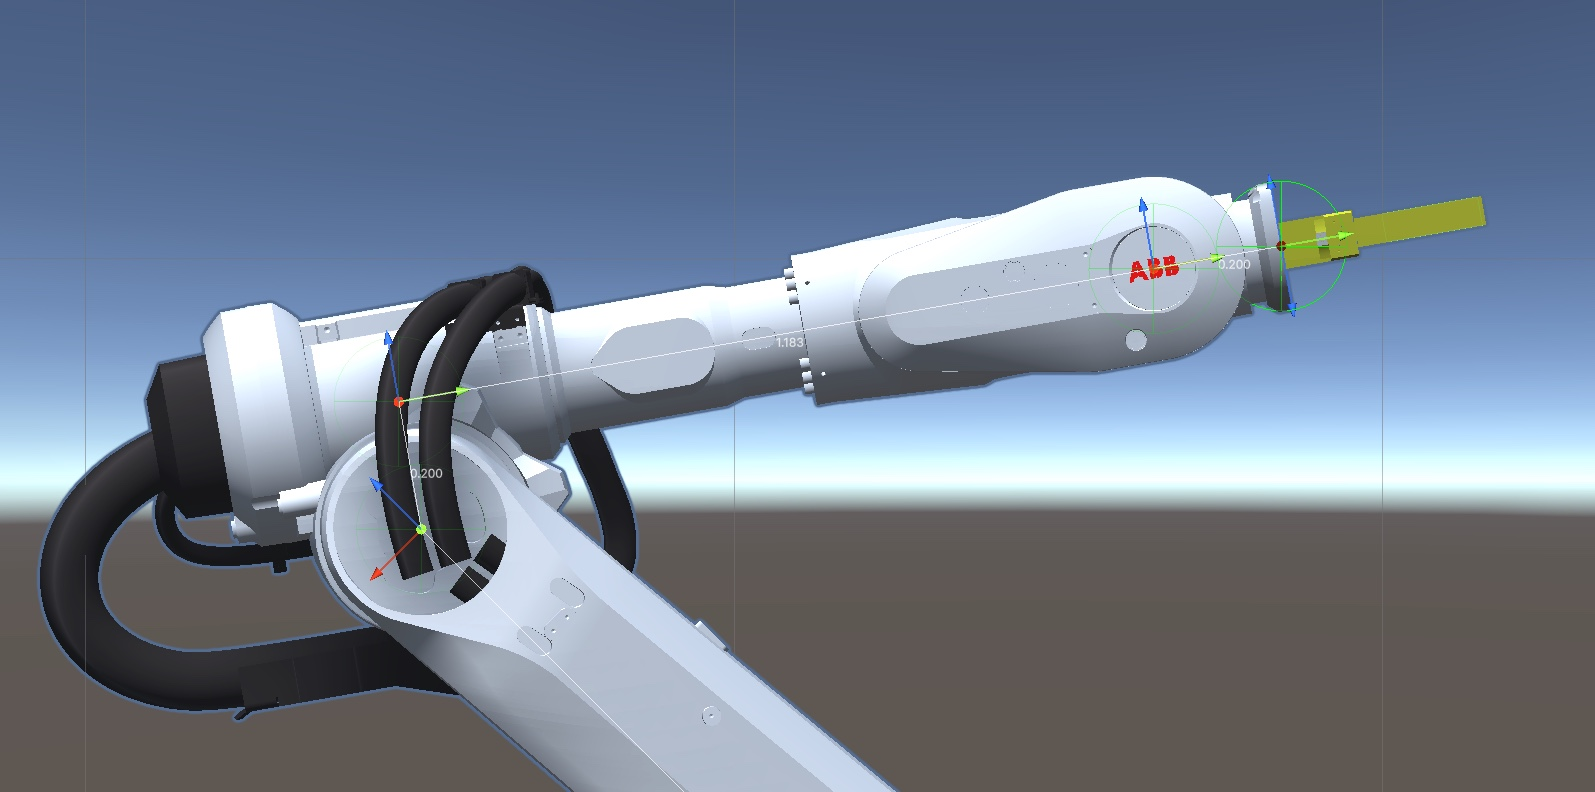
\includegraphics[width=\linewidth]{Figures/wristSingularityScreenshot.jpg}
  \caption{Screenshot einer Handgelenksingularität in Unity mit farbig
  dargestellten Koordinatensystemen der Denavit-Hartenberg-Transformationen }
  \label{figure:wristSingularity}
\end{figure}

\subsubsection{Praktisches Vorgehen}
Nachfolgend werden die Schritte 1 bis 4 zur Prüfung des Vorliegens
einer Singularität dargestellt.

\paragraph{Schritt 1: Positionsberechnung und Achsentransformation}~\\
Die Positionen der relevanten Gelenke werden durch die Anwendung der
Vorwärtstransformation nach Denavit-Hartenberg (DH)
berechnet\vglcite{denavit1955}:
\begin{equation}
  \vec{p}_i = \text{DH}(\theta_1, \ldots, \theta_i) \quad \text{für }
  i = 2, 3, 5
  \label{eq:position_calculation}
\end{equation}

Die Rotationsachsen werden aus den Transformationsmatrizen extrahiert:
\begin{equation}
  \mathbf{z}_i = \mathbf{T}_i[:3, 2] \quad \text{für } i = 1, 4, 6
  \label{eq:axis_extraction}
\end{equation}

\paragraph{Schritt 2: Singularitätsanalyse}~\\
Für jeden Singularitätstyp wird die entsprechende Bedingung überprüft:
\begin{itemize}
  \item \textbf{Schultersingularität:}
    \begin{equation}
      d_{wc} = \sqrt{x_{wc}^2 + y_{wc}^2}
    \end{equation}
    wobei $(x_{wc}, y_{wc})$ die Position des Handgelenkszentrums in
    der XY-Ebene ist.

  \item \textbf{Ellbogensingularität:}
    \begin{equation}
      \theta_{elbow} = \angle(\vec{p}_3 - \vec{p}_2, \vec{p}_5 - \vec{p}_2)
    \end{equation}

  \item \textbf{Handgelenksingularität:}
    \begin{equation}
      c_{46} = |\mathbf{z}_4 \cdot \mathbf{z}_6|
    \end{equation}
\end{itemize}

\paragraph{Schritt 3: Schwellwertvergleich}~\\
\begin{table}[H]
  \centering
  \begin{tabular}{l l l}
    \hline
    \textbf{Singularitätstyp} & \textbf{Beispiel-Schwellwert}      &
    \textbf{Bedingung}                            \\
    \hline
    Schulter                  & $\tau_{\text{shoulder}} = 100$ mm  &
    $d_{wc} < \tau_{\text{shoulder}}$             \\
    Ellbogen                  & $\tau_{\text{elbow}} = 5^{^\circ}$ &
    $\theta_{elbow} < \tau_{\text{elbow}}$ oder   \\
    &                                    & $\theta_{elbow} >
    180^\circ - \tau_{\text{elbow}}$ \\
    Handgelenk                & $\tau_{\text{wrist}} = 5^{^\circ}$ &
    $c_{46} > \tau_{\text{wrist}}$                \\
    \hline
  \end{tabular}
  \caption{Singularitätsschwellwerte und Detektionsbedingungen}
  \label{tab:singularity_thresholds}
\end{table}

\paragraph{Schritt 4: Manipulierbarkeitsberechnung}~\\
Für detektierte Singularitäten wird ein approximierter Manipulierbarkeitsindex
nach Yoshikawa berechnet:

\begin{equation}
  w = \sqrt{\det(\mathbf{J}(\theta)\mathbf{J}^T(\theta))}
  \label{eq:manipulability}
\end{equation}

Ein kleiner Wert von $w$ indiziert die Nähe zu einer singulären Konfiguration.
Das entwickelte Framework implementiert eine winkelbasierte
Singularitätsdetektion, die geometrische Eigenschaften der Roboterkinematik
direkt nutzt, anstatt auf rechenintensive Jacobi-Matrix-Berechnungen angewiesen
zu sein. Die achsenbasierte Methode basiert auf der Erkenntnis, dass
Handgelenks- und Ellbogensingularitäten geometrisch durch die
Kollinearität von Rotationsachsen
charakterisiert werden können. Schultersingularitäten werden analog durch die
Entfernung des ersten Gelenks zum Handgelenkzentrum in der XY-Ebene
festgestellt.

\subsubsection{Konkrete Implementierung der Detektionsmethoden}
\label{sssec:Implementierung_Detektionsmethoden}
Die Implementierung des \texttt{SingularityDetectionMonitor} nutzt die
Vorwärtskinematik des Preliy Flange Frameworks zur Berechnung der
Gelenkpositionen. Die zentrale Methode \texttt{ComputeJointPosition} berechnet
die kartesische Position eines beliebigen Gelenks durch sukzessive Anwendung
der Denavit-Hartenberg-Transformationsmatrizen (vgl.
Abbildung~\ref{listing:forwardKinematic}).

\begin{figure}[H]
  \inputminted[fontsize=\footnotesize]{csharp}{code-snippets/CalculateJointPos.cs}
  \caption{Vorwärtskinematik zur Positionsberechnung}
  \label{listing:forwardKinematic}
\end{figure}

Die Methode \texttt{ComputeJointPosition} in Abbildung
\ref{listing:forwardKinematic} implementiert die klassische
Vorwärtskinematik durch
Multiplikation homogener Transformationsmatrizen. Jede Matrix $\mathbf{T}_i$
wird aus den DH-Parametern $(\alpha_i, a_i, d_i, \theta_i)$ konstruiert, wobei
$\theta_i$ der aktuelle Gelenkwinkel plus einem konstanten Offset ist. Die
resultierende Transformationsmatrix beschreibt die Position und Orientierung des
Gelenks im Basiskoordinatensystem.\\

Das Framework nutzt Unitys \texttt{Matrix4x4}-Klasse für die
Transformationsberechnungen und die \texttt{GetPosition()}-Methode zur
Extraktion der Translationskomponente. Die Koordinatentransformation zwischen
dem DH-Parametersystem und Unitys linkshändigem Y-up Koordinatensystem wird
dabei durch die Methode \texttt{HomogeneousMatrix.CreateRaw()} des
Flange-Frameworks transparent gehandhabt. Das ermöglicht eine nahtlose
Integration der mathematischen Robotik-Konzepte in die Unity-Umgebung, während
die Echtzeitfähigkeit durch eventgetriebene Berechnung gewährleistet ist.
Bei der Detektion einer Singularität bzw. dem Unterschreiten des im Unity-Editor
definierten Grenzwertes wird ein \texttt{SafetyEvent}-Objekt
instanziert und an die
\texttt{SafetyMonitor} Klasse weitergegeben. Darin werden zusätzlich
Event-Metadaten zu den
Daten der Gelenkwinkelabstände ausgegeben. Sobald der
kritische Bereich verlassen wurde, wird ein weiteres
\texttt{SafetyEvent} ausgegeben, um
den Bereich, in welcher die Singularität auftritt, abstecken zu können.


\section{Testumgebung und -setup}
\subsection{Aufbau der Roboterzelle}
\subsection{Implementierung in Unity}
\section{Datenaufzeichung und Logging}
\subsection{JSON-Struktur}
\subsection{Speicherung}
\chapter{Validierungsergebnisse der Testszenarien}
\label{cap:Ergebnisse}

\section{Überblick und Zielsetzung}

In diesem Kapitel werden die Ergebnisse der im vorherigen Kapitel beschriebenen
Implementierung vorgestellt. Im Fokus steht die Überprüfung der vier
entwickelten Safetymodule – Prozessfolgenüberwachung, Kollisionserkennung,
Achsgeschwindigkeits- und Beschleunigungsüberwachung sowie
Singularitätserkennung – innerhalb der aufgebauten Simulationsumgebung. Ziel ist
es zu überprüfen, inwiefern im gewählten Testsetup eine Erkennung von Fehlern in
der Roboterbewegung und Interaktion, welche mit den vier untersuchten Parametern
zusammenhängen, auftreten. iel ist es zu überprüfen, inwiefern im gewählten
Testsetup eine Erkennung von Fehlern in der Roboterbewegung und Interaktion,
welche mit den vier untersuchten Parametern zusammenhängen, auftreten.\\

\noindent
Für jedes Modul wurden gezielte Testfälle definiert, die sowohl korrekte als
auch fehlerhafte Szenarien abbilden, um die Funktionsweise und Zuverlässigkeit
der Module zu überprüfen. Die Ergebnisse werden anhand von Beobachtungen aus der
Simulation, gespeicherten Zustands- und Ereignisdaten sowie grafischen
Darstellungen aufgezeigt. Die Testfälle wurden dabei als Pfade in RobotStudio
definiert. Diese Pfade werden von RobotStudio in RAPID-Code umgewandelt und
gespeichert. Durch die Synchronisation mit dem Controller und dem Setzen des
aktuellen Programms als Standardprogramm lässt sich das Programm in RobotStudio
simulieren. So wurde für jedes Szenario vorgegangen.\\

\noindent
Zur zusätzlichen Validierung wurde ein Experteninterview durchgeführt, in dem
die Testcases vorgestellt und die Funktionsweise des Frameworks diskutiert
wurden. Die Aussagen des Experten werden an geeigneter Stelle in diesem Kapitel
dargestellt und in Kapitel \ref{cap:diskussion} kritisch eingeordnet.
\newpage
\section{Prozessflussüberwachung}
\label{sec:processauswertung}

\subsection{Abwandlung der Prozessfolge}

Die Validierung der Prozessflussüberwachung erfolgt über die Ausführung eines
korrekten Szenarios als auch eines fehlerhaften Szenarios. Der Fehler soll
provoziert werden, in dem das Werkstück abweichend zum in Abbildung
\ref{figure:Prozessfluss} gezeigten gewünschten Ablauf direkt in das zweite
Regal bewegt wird. Semantisch bedeutet dies ein Überspringen der Station
\textit{Machine}. Das soll ein SafetyEvent triggern, sobald das Werkstück im
falschen Regal abgelegt wird.\\

\noindent
\textbf{Korrekter Prozessfluss}
\begin{enumerate}
  \item Bewegung von Home-Position zu linkem Regal
  \item Greifen des Werkstücks
  \item Bewegung zu Maschine
  \item Platzieren des Werkstücks in Maschine
  \item Warten auf Beendigung des Bearbeitungsprozesses in
    Warteposition (Bearbeitung hier nur simuliert)
  \item Bewegen zum Werkstück und Greifen aus Maschine
  \item Bewegung zu rechtem Regal
  \item Platzieren des Objekts in rechtem Regal
  \item Rückkehr zur Home-Position
\end{enumerate}
\begin{figure}[H]
  \centering
  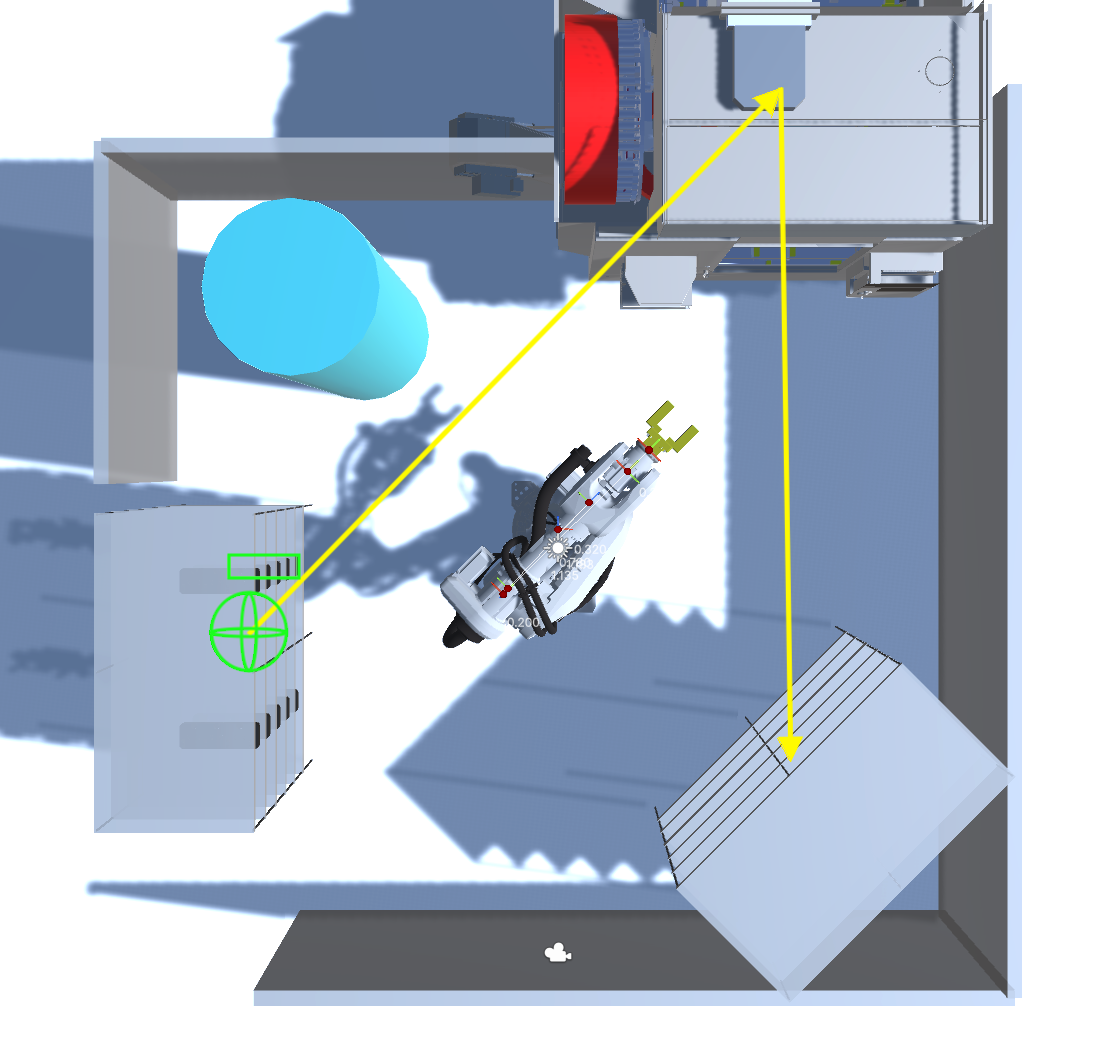
\includegraphics[width=0.7\linewidth]{Figures/Prozessfolge.png}
  \caption{Visuelle Darstellung des Prozessflusses durch Konfiguration der Parts
  und Stations}
  \label{figure:Prozessfluss}
\end{figure}

Im veränderten Prozessfluss wird nun der Schritt der Bearbeitung übersprungen.
Dies kann in der Praxis durch eine inkorrekte Abfolge im Roboterprogrammcode
passieren. Somit ist der veränderte Prozessfluss wie folgt definiert.\\

\noindent
\textbf{Abgewandelter Prozessfluss}
\begin{enumerate}
  \item Bewegung von Home-Position zu linkem Regal
  \item Greifen des Werkstücks
  \item Bewegung zu Maschine
  \item Bewegung zu rechtem Regal
  \item Platzieren des Objekts in rechtem Regal
  \item Rückkehr zur Home-Position
\end{enumerate}

\subsection{Simulationsergebnis}
Wird der korrekte Prozessfluss abgespielt, werden im Bezug auf den
ProcessFlowMonitor keine Ereignisse protokolliert.
Bei der Ausführung des Robotercodes mit verändertem Prozessfluss findet sich in
der nach Beendigung des Programms mit Zeitstempel und Modulname versehenem
JSON-Log ein Eintrag mit einem SafetyEvent getriggert durch den
Process Flow Monitor:
\begin{figure}[H]
  \inputminted[fontsize=\footnotesize]{json}{code-snippets/processflowerror.json}
  \caption{JSON-Log zum Prozessfolgenfehler, Achswinkel wurden im Nachhinein
  entfernt}
  \label{listing:processflowerror}
\end{figure}

\noindent In Abbildung \ref{listing:processflowerror} ist abzulesen, dass der
Fehler hier korrekt erkannt und klassifiziert wurde. Dabei zeigt das Feld
\texttt{description} den genauen Hergang des Events an. Hier wurde eine invalide
Transistion von StorageIn zu StoraeOut versucht. Das Framework erkennt
ebenfalls, welcher Prozessschritt der Richtige gewesen wäre. Ausserdem wird hier
als Violation Type der Type \texttt{SkippedStation} angegeben. Dieser ist als
übersprungene Station zu klassifizieren, was in diesem Fall korrekt ist.
Zusätzlich werden weitere Parameter der Simulation und des Controllers
weitergegeben, unter anderem welches Modul und welche Routine des Moduls zum
Zeitpunkt des Auftretens ausgeführt wurde sowie welcher Programmzeile der
ProgramPointer sich zum Zeitpunkt der Event-Auslösung befand. Durch den Wert des
Keys \texttt{totalSafetyEvents} ist zu erkennen, wie viele Ereignisse bei der
Ausführung vom Programm getriggert wurden. Hier is es lediglich der oben
Genannte.

\section{Auswertung Collision Detection Monitor}
\label{sec:collisionauswertung}

\subsection{Abwandlung des Pfads} Zur Auswertung des Collision Detection
Monitors wurde der oben bereits genannte Prozess genutzt. Anschliessend wurde
der Pfad, auf dem sich der Roboter zwischen seiner Home-Position und dem linken
Regal, in dem er ein Werkstück greifen soll, verändert. Rechts dargstellt in
Abbildung \ref{figure:kollision}, führt der Pfad im Gegensatz zum
kollisionfreien, näher am Roboter verlaufenden Pfad aufgrund des ausladenden
Umschwungs durch die Säulengeometrie. Durch das Abfahren des Pfades gegen den
Uhrzeigersinnd wird proviziert, dass der Roboter sich durch die in Abbildung
\ref{figure:kollision} links blau eingefärbte Säule hindurch bewegen
muss. Die Säule selbst
bekommt den Tag \texttt{Obstacle} und wird durch einen vorhandenen Collider,
welcher den Dimensionen der Säule entspricht, zum Kollisonshindernis.

\begin{figure}[!htb]
  \centering
  \begin{minipage}{.535\textwidth}
    \centering
    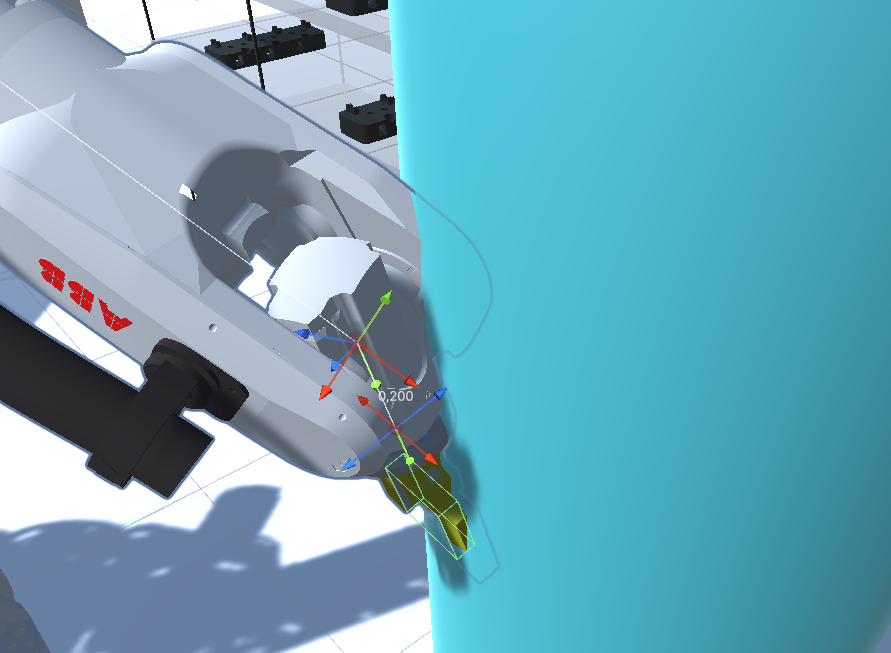
\includegraphics[width=0.9\linewidth]{Figures/CollisionUnity.png}
  \end{minipage}%
  \begin{minipage}{0.465\textwidth}
    \centering
    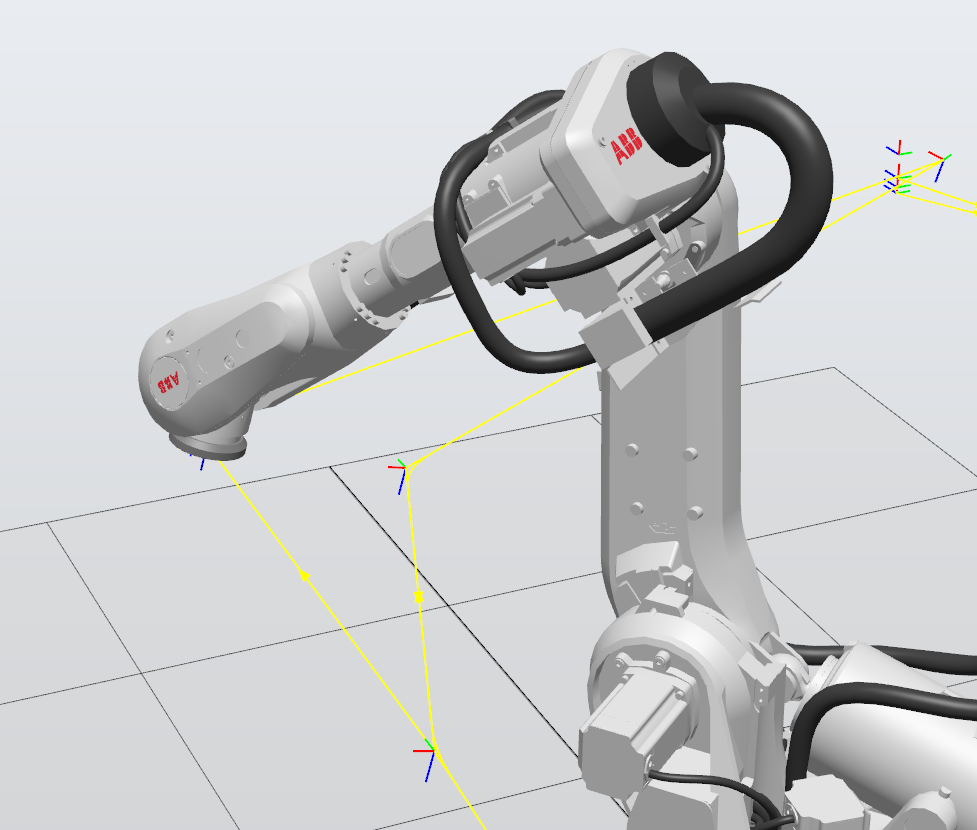
\includegraphics[width=0.9\linewidth]{Figures/CollisionPathRobotStudio.png}
  \end{minipage}
  \caption{Kollision in Unity (links) und zugehörige Position auf Pfad in
    RobotStudio (rechts). Gelenk 4, 5 und 6 sowie Greifer befinden
    sich innerhalb der
  Säulengeometrie.}
  \label{figure:kollision}
\end{figure}

\subsection{Simulationsergebnis}

In Abbildung \ref{listing:collisiondetectionerror} ist der Output nach Kollision
mit der der Säule dargestellet. Dem Event wurden zusätzlich Eventdaten angefügt,
welche hier den Punkt der Kollision im Unity Koordinatensystem als auch die
Entfernung zum Zentrum des kollidierenden Objekts darstellen. Die Kollision wird
somit zuverlässig erkannt. Wichtig ist dabei zu erwähnen, dass die
Kollisionserkennung stark von den verwendeten Collidern abhängt. Hier verwendet
das Framework Mesh-Collider zur genauen Abbildung der Robotergeometrie, das
Kollisionobjekt wird durch einen primitiven zylindrischen Collider definiert.
Beim Outputformat der eventDataJson handelt es sich um string-escaped JSON. Die
Daten sind also als Event-Daten in einem String komprimiert.\\

\begin{figure}[H]
  \inputminted[fontsize=\footnotesize]{json}{code-snippets/collisiondetection.json}
  \caption{JSON-Log zur Kollisionserkennung. Sich wiederholende
    Key-Value Paare wurden
  verkürzt}
  \label{listing:collisiondetectionerror}
\end{figure}

\noindent
Weiterführend ist zu erkennen, dass die Kollison mit verschiedenen Gliedern des
Roboters sequentiell erkannt wird. Sobald der Roboter sich visuell weiter in die
Säule bewegt, wird jeweils bei der Kollison mit einem weiteren Glied eine
weitere Kollision erkannt und ein eigenes Event getriggert. Die Reihenfolge der
Joints in diesem Szenario ist nach eingehender Überprüfung als korrekt zu
bewerten, da die Robotergeometrie dafür sorgt, dass Gelenk 4 deutlich breiter
ist als 5 und 6. Gelenk 5 und 6 sind in die Geometrie von Gelenk 4 eingefasst,
daher kollidert der Roboter inital mit Gelenk 4, bevor eine Kollision an den
kinematisch dahinterliegenden Gelenken erkannt wird.\\

\noindent Weiterführend lässt sich beim Greifen des Werkstücks feststellen, dass
hier ebenfalls eine Kollison erkannt wird: Durch das Greifen des Werkstücks wird
eine falsch-positive Kollison getriggert, da bevor das Werkstück gegriffen wird
und semantisch in die kinematische Kette des Roboters verschoben wird, für einen
kurzen Zeitpunk eine Kollision stattfindet. Ein Beispiel dazu findet sich im
letzten Block von Abbildung \ref{listing:collisiondetectionerror}. Gleiches
lässt sich beim Ablegen desn Werkstücks beobachten. Wichtig zu erwähnen ist der
unterschiedliche EventType, da das Werkstück aufgrund von fehlendem Tag nicht
als kritisch eingestuft wird.

\newpage
\section{Auswertung Singularity Detection Monitor}
\label{sec:singularityauswertung}

\subsection{Künstliche Singularitätserzeugung}
\begin{figure}[H]
  \centering
  \includegraphics[width=0.7\textwidth]{figures/wristSingularity.png}
  \caption{Pose in Unity, bei der eine Wrist-Singularität mit
  ($\theta_{5} \approx 0^\circ$) entsteht}
  \label{fig:wristSingularity}
\end{figure}

Zur Untersuchung der Singularitätserkennung wurde in RobotStudio ein
Szenario erstellt,
das gezielt eine Wrist-Singularität provoziert. Dabei wurde der
Roboter in eine Pose
geführt, in der die Achsen~4 und~6 nahezu kollinear verlaufen und
somit die Bedingung
$\theta_{5} \approx 0^\circ$ erfüllt ist. Die Pose ist in Abbildung
{fig:wristSingularity} zu erkennen, hier befindet sich der Roboter nach dem
Greifen des Werkstücks auf dem Weg zum rechten Regal, muss sich für das
Platzieren des Werkstücks im Regal jedoch umorienten. So kommt die Singularität
zustande.

\subsection{Simulationsergebnis}
\begin{figure}[H]
  \inputminted[fontsize=\footnotesize,breaklines]{json}{code-snippets/singularityerror.json}
  \caption{Gekürzter Auszug der in Unity aufgezeichneten Safety
  Events zur Wrist-Singularität}
  \label{lst:singularity_json}
\end{figure}

\noindent
Die vom Monitor in Unity aufgezeichneten Safety Events sind in
Abbildung~\ref{lst:singularity_json} als gekürzter Auszug
dargestellt. Es werden sowohl
das \enquote{Entering}- als auch das \enquote{Exiting}-Ereignis
erfasst, jeweils mit den
zugehörigen Gelenkwinkeln und einem berechneten
Manipulierbarkeitswert. Nicht relevante
Felder des Snapshots wurden entfernt, da die Gelenkwinkel bereits im
\texttt{eventDataJson}
enthalten sind. Zusätzliche Informationen wurden mit \texttt{"[...]"}
abgekürzt.\\

\noindent
Die Analyse der Ereignisse zeigt, dass der Monitor den Eintritt in
die Wrist-Singularität
bei einer Gelenkkonfiguration von etwa
$[-82.7, -6.9, 36.6, -112.8, -4.9, -153.5]^\circ$ registrierte. Der berechnete
Manipulierbarkeitswert lag hier bei $w \approx 0.19$. Beim Verlassen der Pose
($[-91.8, -8.3, 37.8, -91.3, 5.2, -182.6]^\circ$) wurde das
\enquote{Exiting}-Ereignis
ausgegeben, wobei der Manipulierbarkeitswert mit $w \approx 0.20$
ebenfalls sehr niedrig blieb.
Die Ereignisse decken sich mit dem in RobotStudio provozierten
Szenario und markieren den
Übergang in und aus einer singulären Konfiguration.
Zur Detektion von Singularitäten anderen Typs (hier Schulter- und
Ellbogensingularitäten) wird das gleiche Verfahren angewendet. Hier decken sich
die Ergebnisse mit den oben Beschriebenen.

\section{Auswertung Joint Dynamics Monitor}
\label{sec:Analyse_Sicherheit}

\subsection{Überhöhung der Gelenkgeschwindigkeiten}

Der \textit{Joint Dynamics Monitor} erfasst kontinuierlich die Dynamik der sechs
Roboterachsen. Die Implementierung in Unity basiert auf den vom digitalen
Zwilling gestreamten Gelenkwinkeln, aus denen Geschwindigkeiten und
Beschleunigungen differenziell berechnet werden. Zur Signalanalyse werden
mehrere Mechanismen kombiniert, darunter exponentielle Glättung sowie
Fenster-basiertes Mittel zur Dämpfung von Ausreißern. Zusätzlich wird ein
Sicherheitsfaktor von 0{,}8 auf die in RobotStudio spezifizierten Maximalwerte
angewendet, sodass die Schwellwerte im Monitor niedriger liegen als die realen
physikalischen Limits (vgl. Implementierung in
\texttt{JointDynamicsMonitor.cs}). Hier wird mittels des Befehl \texttt{v7000}
im RAPID-Code in RobotStudio die Geschwindigkeit auf den programmierbaren
Maximalwert gesetzt. Dies wurde an zwei Stellen der Roboterbewegung umgesetzt:
Bei der Bewegung von der Home-Position zum linken Regal und bei der Bewegung
nach dem Greifen des Werkstücks zur Maschine. Als primäre Drehachse ist hier
eine Überhöhung der Geschwindigkeit von Gelenk 1 (zentrale horizontale Drehachse
des Roboters) zu erwarten.

\subsection{Simulationsergebnis}

Während der Testsimulation wurden durch den Monitor zwei Überschreitungen der
Geschwindigkeitsgrenzen auf \textbf{Joint 1} registriert. Diese Ereignisse sind
in der aus Unity aufgezeichneten Logdatei dokumentiert. Ein Auszug ist in
Abbildung~\ref{lst:jointdynamics_json} dargestellt. Dort wird jeweils die
Überschreitung der Geschwindigkeit und das nachfolgende
\enquote{resolved}-Ereignis vermerkt, zusammen mit dem aktuellen
Gelenkwinkelzustand des Roboters.

\begin{figure}[H]
  \inputminted[fontsize=\footnotesize,breaklines]{json}{code-snippets/jointdynamicserror.json}
  \caption{Gekürzter Auszug der in Unity aufgezeichneten Safety
  Events des Joint Dynamics Monitor, Ereignis widerholt sich}
  \label{lst:jointdynamics_json}
\end{figure}

Zum Vergleich wurden die Gelenkwinkel aus RobotStudio exportiert und
anhand der berechneten
Achsgeschwindigkeiten ausgewertet. Abbildung~\ref{fig:jointdynamics}
zeigt die Ergebnisse:
Im oberen Diagramm sind die Achswinkel aller sechs Gelenke
dargestellt (J1 hervorgehoben in rot),
darunter die berechneten Geschwindigkeiten mit markierten Schwellwertbereichen.
Die rot eingefärbten Abschnitte kennzeichnen Intervalle, in denen die
aus RobotStudio
exportierten Daten die definierte Grenze von $\pm 50\,^\circ$/s überschreiten.
Die blau markierten Bereiche repräsentieren die durch den Monitor in
Unity ausgegebenen
Safety Events.
Zu erkennen ist eine starke Überschneidung der Bereiche.
Weiterführend zeichnet sich vor allem in der zweiten
Geschwindigkeitsüberschreitung eine Verzögerung beim Ein- und Austritt in den
kritischen Zustand ab. Die Events in Unity werden hier zeitverzögert
weitergegeben.

\begin{figure}[H]
  \centering
  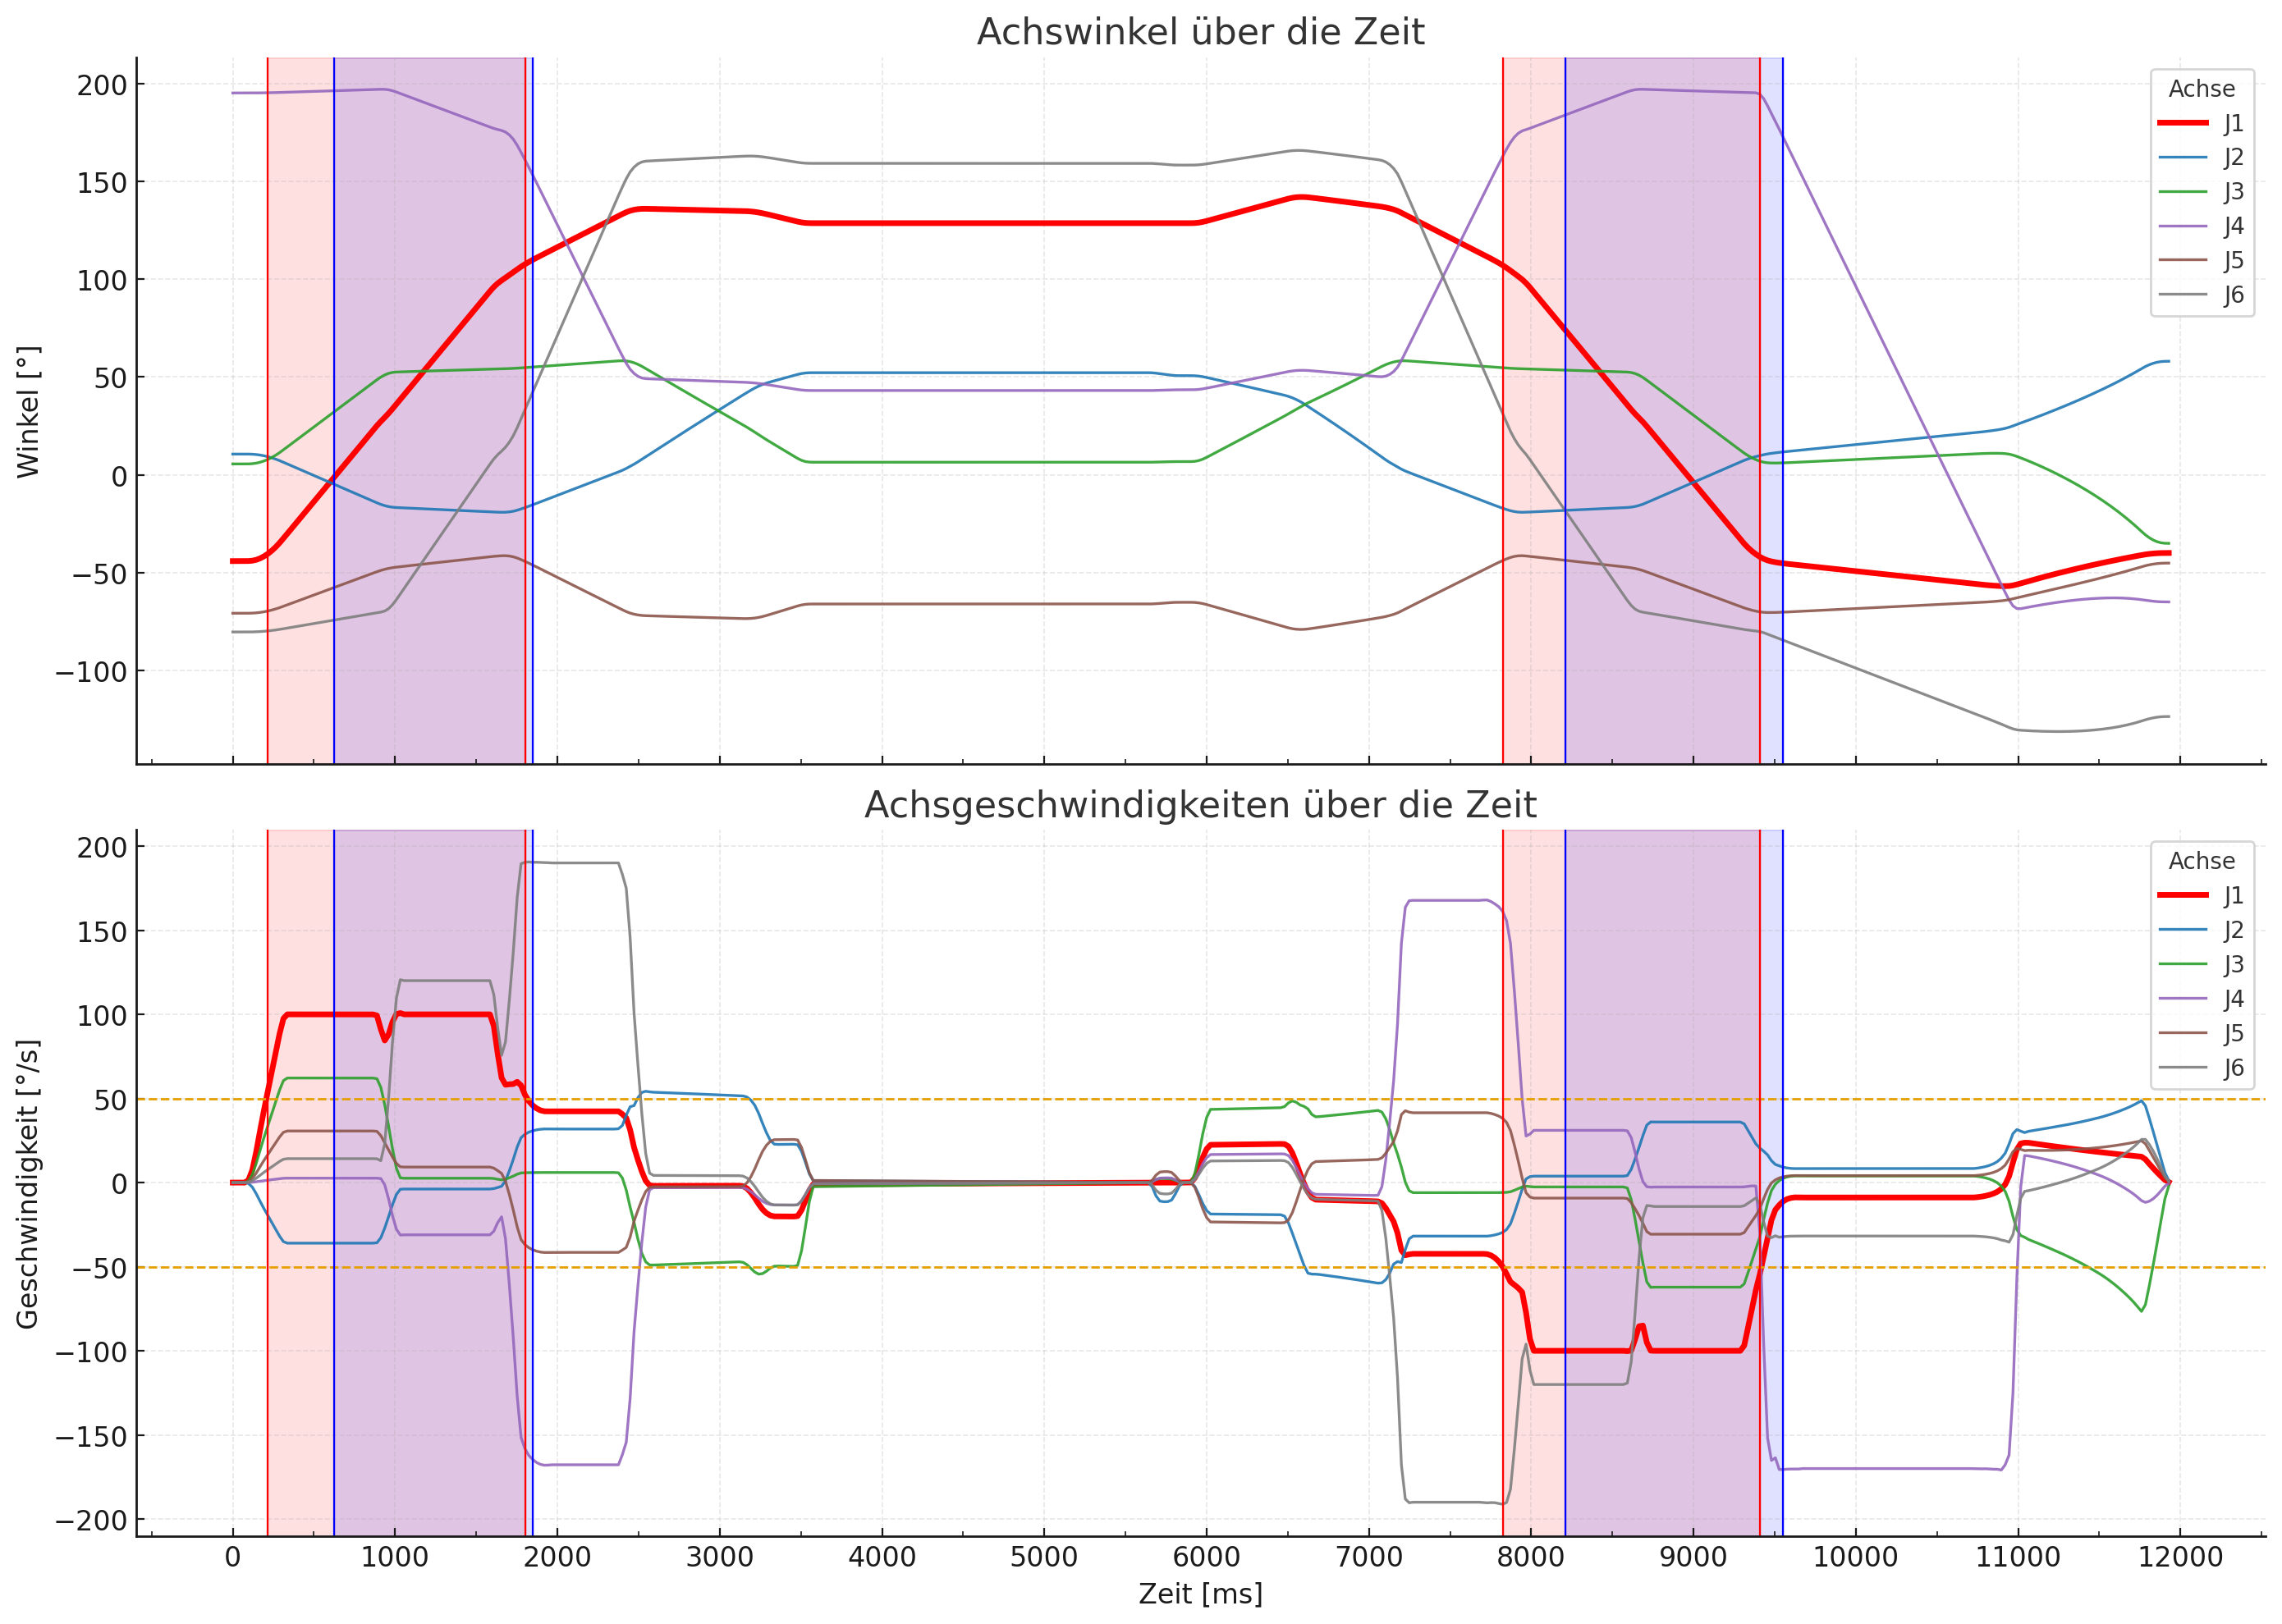
\includegraphics[width=\textwidth]{Figures/achsgeschwindigkeitPlot.png}
  \caption{Achswinkel (oben) und Achsgeschwindigkeiten (unten) mit markierten
    Bereichen (rot: Schwellenübertritte in den Rohdaten, blau: Safety
  Events aus Unity).}
  \label{fig:jointdynamics}
\end{figure}

Eine Gegenüberstellung der Zeitintervalle ist in
Tabelle~\ref{tab:jointdynamics} enthalten.
Dort werden die Start- und Endzeitpunkte der Abschnitte, die Dauer
sowie die Gelenkwinkel
und -geschwindigkeiten an diesen Punkten angegeben. Anhand dieser
Darstellung wird sichtbar,
dass die blau markierten Safety Events zeitlich nach den rot
markierten Schwellenübertritten
liegen. Die in Tabelle~\ref{tab:jointdynamics} und Abbildung
\ref{fig:jointdynamics} dargestellten Intervalle wurden ermittelt,
indem die aus RobotStudio exportierten Gelenkwinkel mit den in den Safety Events
gespeicherten Zuständen vergleichar sind. Dazu wurde der euklidische
Abstand zwischen
den Vektoren der Achswinkel berechnet, um den jeweils nächstliegenden
Zeitpunkt in
den Referenzdaten zu bestimmen. Auf diese Weise lassen sich die vom
Monitor in Unity
gemeldeten Ereignisse mit den in den Rohdaten beobachteten Schwellenübertritten
korrelieren.

\begin{table}[H]
  \centering
  \small
  \begin{tabularx}{\textwidth}{lrrrrrrX}
    \toprule
    Typ               & Start [ms] & Ende [ms] & Dauer [ms] & Start
    J1 [\textdegree] & Ende J1 [\textdegree] \\
    \midrule
    Dynamik (rot)     & 216        & 1800      & 1584       & -40.35
    & 107.62                \\
    Zielwinkel (blau) & 624        & 1848      & 1224       & -1.25
    & 109.89                \\
    Dynamik (rot)     & 7824       & 9408      & 1584       & 107.08
    & -41.88                \\
    Zielwinkel (blau) & 8208       & 9552      & 1344       & 74.15
    & -45.24                \\
    \bottomrule
  \end{tabularx}
  \caption{Zeitintervalle und Zustände der Joint-Dynamics-Auswertung}
  \label{tab:jointdynamics}
\end{table}

\section{Validierung durch Experteninterview}

Im Rahmen der Ergebnisdarstellung wurde ein Experteninterview mit Daniel Syniawa
(M.Sc.) durchgeführt. Ziel war es, die
Funktionsfähigkeit des Frameworks praxisnah zu validieren und Einschätzungen zur
industriellen Einordnung zu gewinnen. Das Interview diente ausschließlich der
\emph{deskriptiven} Ergänzung der Ergebnisse; eine vertiefte Interpretation
erfolgt in Kapitel~\ref{cap:diskussion}.

\subsection{Vorgehen und Gegenstand}

Im Interview wurden die Software und ihre Architektur vorgestellt. Anschließend
wurden die in Kapitel~4 beschriebenen Testfälle gemeinsam in \emph{RobotStudio}
nachvollzogen: Der Roboter führte die Szenarien aus, während parallel beobachtet
wurde, ob und wie die Module Ereignisse auslösen und ob diese im Logging erfasst
werden. Damit wurde die grundsätzliche Funktionsweise des Frameworks
demonstriert (Auslösen von Safety-Events, Erzeugung von JSON-Logs mit
Programmkontext).

\subsection{Beobachtungen}

Prinzipiell konnte ein schnelles Verständnis für die Anwendung des Frameworks
und dessen Funktionsweise gewonnen werden. Bei der Testung der Fälle wurde der
praktische Nutzen der abgespeicherten JSON-Logs hervorgehoben: Für jedes
Ereignis liegen der aktuelle Programmzeiger, das aktuell ausgeführte Programm
sowie die relevante Roboterpose bzw.\ Kontextinformationen vor. Dies erleichtert
die Fehlersuche und macht die Analyse auch für weniger erfahrene Anwender
nachvollziehbar.

\subsection{Hinweis zur Evaluationsmethodik}

Für eine belastbare Evaluation schlug Syniawa vor, die Leistung des Frameworks
\emph{quantitativ} gegen manuelle Verfahren zu vergleichen. Konkret: Wie schnell
findet eine Person den Fehler (z.\,B.\ Auftreten einer Singularität) im
RAPID-Code in \emph{RobotStudio} im Vergleich zur Erkennung durch Ausführung und
Logging im Framework? Ein solcher Vergleich wäre mit erheblichem Aufwand
verbunden, würde aber die Einordnung der Wirksamkeit deutlich schärfen.

\subsection{Einordnung des Robotersimulations-Ökosystems}

Syniawa wies darauf hin, dass die aktuelle Werkzeuglandschaft stark proprietär
geprägt ist und es nur wenige plattformübergreifende Lösungen mit integrierter
Physik gibt. Häufig ist bereits die stabile Anbindung eines Roboters
herausfordernd; Simulation in \emph{RobotStudio} erfordert viel Expertenwissen
und Zeit. Die \emph{Robot Web Services} (RWS) seien komplex und eher knapp
dokumentiert; insgesamt sei die Nutzerbasis in diesem Bereich klein. Diese
Beobachtungen unterstreichen die Relevanz eines modularen, erweiterbaren
Ansatzes wie in dieser Arbeit umgesetzt.

\subsection{Zusammenfassung}

Das Interview bestätigte die grundsätzliche
Funktionalität des Frameworks in den demonstrierten Testfällen und
identifizierte einen klaren Pfad für eine zukünftige, quantitative Evaluation.
Zudem wurde der praktische Mehrwert der strukturierten Logs (Programmzeiger,
laufendes Programm, Pose/Kontext) betont. Die Einordnung der industriellen
Robotersimulationslandschaft liefert den Rahmen, in dem die
vorgestellten Ergebnisse zu
sehen sind.

\section{Zusammenfassung der Ergebnisse}

Die Ergebnisse zeigen, dass die in Unity implementierten Monitore in allen
Testfällen die in RobotStudio provozierten Szenarien widerspiegeln konnten.
Dabei wurde deutlich, dass sich für jedes Modul charakteristische Muster im
Logging abzeichnen: Prozessabweichungen wurden sequenziell dokumentiert,
Kollisionen mit Schweregraden versehen, Singularitäten mit Gelenkwinkeln und
Manipulierbarkeitswerten erfasst, und Geschwindigkeitsverletzungen durch
Event-Paare (exceeded/resolved) gekennzeichnet.\\

\begin{table}[H]
  \centering
  \small
  \begin{tabularx}{\textwidth}{lXX}
    \toprule
    \textbf{Monitor}      & \textbf{Getestetes Szenario}
    & \textbf{Erkannte Ereignisse / Beobachtungen}
    \\
    \midrule
    Process Flow          & Ablauf mit bewusst fehlerhafter
    Reihenfolge der Operationen                                &
    Abweichung von der erwarteten Sequenz korrekt erkannt, Events
    dokumentieren Verletzung der Prozessfolge.
    \\
    \addlinespace
    Collision Detection   & Simulation mit Kollision zwischen Greifer
    und Werkstück bzw. Störkörper                    & Mehrere
    Kollisionen aufgezeichnet, inklusive beteiligter Objekte; Events
    mit Schweregrad (critical/warning) unterschieden.                 \\
    \addlinespace
    Singularity Detection & Pose in RobotStudio, die eine
    Wrist-Singularität ($\theta_{5} \approx 0^\circ$) provoziert &
    ENTERING- und EXITING-Events erfasst; Gelenkwinkel und
    Manipulierbarkeitswerte im JSON protokolliert; Szenario deckt
    sich mit RobotStudio. \\
    \addlinespace
    Joint Dynamics        & Bewegung mit Überschreitung der
    Geschwindigkeitsgrenzen auf J1 ($\pm 50^\circ$/s)          & Zwei
    Event-Paare (exceeded/resolved) aufgezeichnet; Verzögerung
    zwischen Schwellenübertritt (Rohdaten) und Event (Monitor)
    sichtbar.       \\
    \bottomrule
  \end{tabularx}
  \caption{Übersicht der getesteten Monitore, Szenarien und erkannten
  Ereignisse im Ergebnisteil}
  \label{tab:monitor_overview}
\end{table}

\noindent
Die Übersicht in Tabelle~\ref{tab:monitor_overview} verdeutlicht die
Unterschiede
zwischen den Monitoren hinsichtlich Art der Szenarien und Form der
erfassten Events.
Auffällig ist, dass sich in einigen Fällen eine zeitliche Verzögerung zwischen
den in den Rohdaten beobachteten Zuständen und den vom Monitor generierten
Ereignissen zeigt. Diese Beobachtung ergibt sich aus den in Kapitel~3
beschriebenen
Mechanismen (z.\,B. Glättung, Abtastrate).\\

\noindent
Im nächsten Abschnitt wird ein Experteninterview herangezogen, um die hier
dargestellten Ergebnisse einzuordnen und im Hinblick auf ihre Relevanz für
praktische Anwendungen zu reflektieren.

\chapter{Diskussion}
\label{cap:diskussion}

\section{Einleitung} In diesem Kapitel werden die in
Kapitel~\ref{cap:Ergebnisse} präsentierten
Ergebnisse kritisch reflektiert und in den fachlichen Kontext eingeordnet. Im
Zentrum stehen die Gesamtarchitektur des Frameworks und die vier implementierten
Safetymodule. Ergänzend wird ein Experteninterview mit Daniel Syniawa
herangezogen, in dem die Software, die Architektur sowie konkrete Testcases in
RobotStudio gemeinsam betrachtet wurden. Ziel ist es, die Stärken und Grenzen
der Arbeit transparent zu machen und konkrete Ansatzpunkte für zukünftige
Arbeiten zu identifizieren.

\section{Diskussion des Frameworks}

Die Architektur hat sich als tragfähige Grundlage erwiesen: Durch den
adapterbasierten Zugriff auf die Roboterschnittstelle (z.\,B. ABB Robot Web
Services) und eine konsequent \emph{event-getriebene} Struktur konnten
Safetymodule unabhängig voneinander entwickelt und über ein gemeinsames
Interface in das \emph{RobotSystem} integriert werden. Das Event-System
(Observer-Pattern) entkoppelt Erkennung und Verarbeitung; die JSON-basierte
Persistenz vereinfacht Nachvollziehbarkeit und Weiterverarbeitung. Positiv
wirkte sich zudem die Nutzung der Denavit–Hartenberg-Parameter aus, die eine
konsistente kinematische Modellierung verschiedener Robotermodlle erlaubt.\\

\noindent Gleichzeitig bleiben offen, inwiefern einzelne Simulationsparameter
oder Modellierungsentscheidungen in Unity bei hochkomplexen Geometrien eine
Limitation darstellen \emph{könnten}. Die Unity-Engine bietet hier zwar eine
Grundlage physischer Modellerung, abschliessende Aussagen zur Genauigkeit in
sehr dynamischen oder kleinschrittigen Prozessen können aber nicht getrofen
werden. Diese Aspekte wurden nicht systematisch untersucht und markieren Raum
für künftige Studien.\\

\noindent Das Experteninterview mit Daniel Syniawa ordnet die Arbeit in die
Praxis ein: Er bestätigte, dass es insgesamt nur wenige plattformübergreifende
Werkzeuge mit integrierter Physik gibt und dass die Tool-Landschaft stark
proprietär geprägt ist. Nach seiner Erfahrung ist bereits die stabile
Inbetriebnahme und Anbindung von Robotern für viele Firmen aufwendig;
physikalische Simulation mit einer Modellerung des Arbeitsraumes in RobotStudio
sowie die Auswertung der hier untersuchten Parameter ist nur in begrenztem
Umfang möglich und benötigt beträchtliches Expertenwissen und Zeit. Syniawa wies
außerdem darauf hin, dass Services proprietär Hersteller wie die RobotStudio-API
(Robot Web Services) nicht trivial in der Anwendung sind, oft schlecht
dokumentiert und auf eine insgesamt kleine Nutzerbasis trifft. Auch das lässt
sich im Rahmen der Entwicklung dieses Frameworks bestätigen.

Als hilfreich lässt sich ausserdem der Output des JSON-basierten Loggings
werten: Syniawa spricht hier vor allem von den mit einem SafetyEvent zusammen
herausgegebenen Metadaten zum aktuellen Stand des Programmzeigers und
der aktuellen
ausgeführten Routine. Dies stellt einen vielversprechenden Ansatz zum Debugging
im Roboterprogrammcode dar, welcher manuell mit deutlich mehr Aufwand verbunden
wäre. Hier gilt es weiter zu evaluieren, inwiefern sich dies quantitativ
beschreiben lässt, so Syniawa.

\section{Diskussion der Safetymodule}

\subsection{Prozessfolgenüberwachung}

Das Modul erkennt Abweichungen in der vorgesehenen Reihenfolge zuverlässig,
sofern Stationen korrekt modelliert und ausgelöst werden. Nicht abgedeckt sind
Konstellationen, in denen ein Werkstück \emph{zwischen} zwei Stationen
unbeabsichtigt abgelegt oder verloren wird, ohne dass eine Station detektiert
wird. Die Praxistauglichkeit hängt damit von der Qualität der
Prozessmodellierung und der Art des Prozesses ab. Im aktuellen Fokus stand hier
ein sequentieller Prozess, die Literatur beschreibt hier im Kontext
industrieller Fertigung jedoch mehrere Prozessarten und theoretische
Modellierungsansätze. Im Interview wurde die grundsätzliche Relevanz dieses
Moduls bestätigt; zugleich wird deutlich, dass die industrielle Praxis oft
komplexere Ablaufmodelle erfordert.

\subsection{Kollisionserkennung}

In der Simulation wurden die vorgesehenen Kollisionsfälle erkannt; zugleich
traten Fehlalarme auf, insbesondere beim Greifen und Loslassen von Werkstücken.
Wie stark Modellierungsdetails oder Simulationsparameter das Verhalten in
Grenzfällen beeinflussen, wurde in dieser Arbeit nicht systematisch untersucht
und ist als potenzielle Limitation zu betrachten. Weiterführend ist die
Genauigkeit der Modellierung der Meshes des Roboters und der Umgebung hier
essentiell: Unity modelliert konvexe Meshes, welche die räumlichen Grenzen
darstellen mit maximal 255 Kanten. Daher kann es passieren, dass die
tatsächliche Topologie des Robotermodells vom Kollisionskörper abweicht.
Insgesamt liefert das Modul einen belastbaren Proof-of-Concept, dessen
Generalisierung im Rahmen weiterführender Evaluierungen zu prüfen ist.

\subsection{Achsgeschwindigkeiten und -beschleunigungen}

Grenzwertverletzungen wurden zuverlässig detektiert. In den Ergebnissen zeigte
sich allerdings ein zeitlicher Versatz zwischen den in RobotStudio vorliegenden
Referenzdaten und der Detektion in Unity: Überschreitungen wurden etwas später
erkannt und endeten geringfügig später. Dieser Versatz ist plausibel auf
Aktualisierungsrate und eingesetzten Glättungsalgorithmus zurückzuführen, dessen
Parameter konfigurierbar sind. Ob dadurch ein Versatz mit den in der Praxis
vom Roboter gefahrenen Achsgeschwindigkeiten und -beschleunigungen
entsteht, lässt sich hier
nicht abschliessend bewerten.

\subsection{Singularitätserkennung}

Die gewählte, winkelbasierte Heuristik funktionierte für den betrachteten
Roboter, ist jedoch nicht universell. Alternativ bieten sich Kennzahlen an, die
näher an der Kinematik operieren, etwa das Manipulability-Maß (Yoshikawa) oder
der kleinste Singulärwert der Jacobi-Matrix als Abstandsmaß zur Singularität.
Eine generische, Jacobian-basierte Methode zur Erkennung von
Freiheitsgradverlusten wurde implementiert, im Rahmen der vorliegenden Tests
jedoch nicht eingesetzt; eine Erweiterung auf andere Roboter wäre möglich, wurde
aber nicht vorgenommen.

Im Interview formulierte Syniawa einen pragmatischen Maßstab für die Evaluation:
Für eine belastbare Beurteilung wäre ein direkter Vergleich mit manuellem
Debugging in RobotStudio sinnvoll, also ein Messaufbau, der die Zeit bis zur
Fehlerlokalisierung im RAPID-Code der Zeit gegenüberstellt, die das Framework
über Ausführung und Logging benötigt. Zugleich hob er hervor, dass die
automatische Bereitstellung von Programmzeiger, aktueller Pose und Kontext im
Event-Log eine erhebliche Arbeitserleichterung darstellt und die Analyse
prinzipiell auch weniger erfahrenen Anwendern ermöglicht.

\section{LLM-gestützte Rückkopplung auf Basis der Safety-Events}

Die Ergebnisse zeigen, dass das Framework Fehlerzustände konsistent
und kontextreich protokolliert: Für jedes Ereignis liegen
Aktuelle Bewegungs- und Programmdaten, beispielsweise das aktuelles
Modul, Routine,
Programmzeile sowie Motordaten und Achswinkel vor. Hinzu kommen
event-spezifische Felder im \texttt{eventDataJson}, etwa
Kollisionspunkt und Distanz oder Gelenkwinkel und
Manipulierbarkeitswert bei Singularitäten\footnote{Vgl. u.\,a.
  Process-Flow-Event inkl.\ Programmpointer und RobotStateSnapshot
  sowie die Beschreibung des JSON-Aufbaus; Kollisionsevents mit
  \texttt{collisionPoint} und Distanz; Singularitätsevents mit
  Gelenkwinkeln und Manipulierbarkeitswert; Joint-Dynamics-Events als
\enquote{exceeded}/\enquote{resolved}.}. Diese maschinenlesbare
Struktur eignet sich unmittelbar als gezielter Eingabekontext für
generative Modelle: Der Fehler wird präzise beschrieben, der
relevante Zustandsausschnitt ist enthalten, und die Semantik stammt
aus den domänenspezifischen Monitoren. Das bietet eine gute Basis, um Code-
oder Pfadänderungen vorzuschlagen und anschließend identisch zu
verifizieren.

Operativ lässt sich darauf ein kurzer Iterationszyklus aufbauen: Aus
einem fehlgeschlagenen Lauf durch Nutzer- oder LLM-generierten
Roboterprogrammcode wird ein kompakter Fehlerkontext aus
gebildet und an ein LLM übergeben: Das
LLM liefert einen minimalen Änderungsvorschlag am Robotercode
bzw.\ an der Pfaddefinition und durch die Re-Simulation kann eine erneute
Prüfung des Codes stattfinden. Die Akzeptanzkriterien für eine erfolgreiche
Behebung des Fehlers beispielsweise mit dem minimalen Achswinkel bereits
im Rahmen der Eventdaten und Monitorlogik im System vor wodurch die
Bewertung reproduzierbar bleibt.
Damit kann das Framework als
Schnittstelle zwischen realitätsnaher Ausführung und
LLM-gestützter Verbesserung dienen. Praktisch sind drei Punkte entscheidend
und aus den Ergebnissen ableitbar: erstens ein schlanker, stabiler
Prompt-Ausschnitt aus genau den Feldern, die im Logging ohnehin
verfügbar sind (z.\,B.\ Programmpointer, Gelenkwinkel,
Kollisionspunkt), zweitens feste Akzeptanzregeln in der Simulation,
drittens Versionierung und Wiederholbarkeit der Läufe. Auf dieser
Basis lässt sich in zukünftiger Arbeit untersuchen, in welchem Umfang
sich Fehlerquote und Nachbearbeitungszeit durch die Rückkopplung
tatsächlich reduzieren – die in den Ergebnissen sichtbaren Muster wie
liefern bereits geeignete Zielgrößen.

\section{Reflexion des eigenen Vorgehens}

Die Entwicklung folgte bewusst einem iterativen Vorgehen: von einem kleinen
Testfall hin zu einer breiteren Abdeckung, mit Zwischenstufen des Refactorings.
Dieses Vorgehen erwies sich als geeignet, um Architekturentscheidungen
(Adapter/Observer) empirisch zu validieren. Rückblickend entstanden stellenweise
Komponenten, die für den unmittelbaren Use-Case komplexer waren als nötig;
gleichwohl war die iterativ-explorative Herangehensweise im Kontext einer
Framework-Entwicklung zweckmäßig und hat zur jetzigen Struktur geführt.

\section{Grenzen und Generalisierbarkeit}

Die vorliegende Arbeit wurde in der Simulation evaluiert; Echtzeitverhalten,
Sensitivität gegenüber Simulationsparametern sowie Übertragbarkeit auf weitere
Roboter wurden nicht systematisch untersucht. Darüber hinaus beschränkt sich die
Adaptervalidierung auf ABB Robot Web Services. Das Interview verdeutlicht, dass
proprietäre Ökosysteme, komplexe Schnittstellen und eine kleine Nutzerbasis
zusätzliche Hürden für Verallgemeinerung und Transfer darstellen. Diese Punkte
markieren bewusste Grenzen des aktuellen Stands und leiten unmittelbar zu
Folgestudien über.

\chapter{Fazit und Ausblick}
\label{cap:Fazit}

\section{Zusammenfassung}

Das entwickelte Framework demonstriert die Machbarkeit eines modularen,
eventgetriebenen Ansatzes für sicherheitsrelevante Überwachungsaufgaben in der
Roboterprogrammierung. Die Module erfüllten ihre Kernfunktionen, zugleich wurden
klare Erweiterungspfade sichtbar. Das Experteninterview mit Daniel Syniawa
bestätigte Relevanz und Nutzen des Ansatzes und unterstrich die praktischen
Hürden einer stark proprietären Werkzeuglandschaft. Insgesamt stellt die Arbeit
einen belastbaren Proof-of-Concept dar, der durch quantitative Evaluationen und
architektonische Erweiterungen in Richtung eines praxistauglichen Systems
weitergeführt werden kann.

\section{Ausblick}

Aus den Diskussionen ergeben sich zwei unmittelbare Schienen:
Erstens eine \emph{quantitative} Evaluation, die die Leistungsfähigkeit des
Frameworks systematisch gegen manuelle Verfahren stellt. Mögliche Metriken
umfassen etwa Erkennungszeit, Zuverlässigkeit (Recall) der Detektion und
Fehlalarmrate; für die Dynamiküberwachung sind zudem akzeptable Toleranzbänder
zu definieren und transparent zu begründen. Zweitens eine
\emph{architektonische} Weiterentwicklung: engere Kopplung an
Controllerschnittstellen, Erweiterung auf weitere Herstelleradapter sowie die
Prüfung echtzeitnaher Ausführungsumgebungen.

Langfristig eröffnet die strukturierte JSON-Ausgabe eine Brücke zu
automatisierten Analyse- und Korrekturprozessen. Eine naheliegende Linie ist die
Einbindung von Large Language Models (LLMs), die auf Basis von Logdaten und
Layoutinformationen Roboterprogramme analysieren und Verbesserungsvorschläge
generieren. In einem nächsten Schritt ließe sich dies als MCP-Server
konzipieren, der Rückmeldungen zyklisch in das Framework einspeist und damit den
Bedarf an tiefem Expertenwissen reduziert, ohne den Sicherheitsanspruch zu
unterlaufen.


% Literaturverzeichnis
\printbibliography

% Anhang
\chapter*{Anhang}
\label{cap:Anhang}

\addcontentsline{toc}{chapter}{Anhang} 

%%%%%%%%%%%%%%%%%%%%%%%%%%%%%%%%%%%%%%%%%%%%%%%%%%%%%%%%%%%%%%%%%%%%%%%%%%%%%%%%%%%%%%%%%%%%%%%%%%%%%%%%%%%%%%%%%%%%%%%%%%%%%%%%%%%%%%%%%%%%%%%%%%%%%%%%%%%%%%%%%%%%%%%%%%%%%%%%%%%%%%%%%%%%%%%%%%%%%%%%%%%%%%%%%%%%%%%%%%%%%%%%%%%%%%%%%%%%%%%%%%%%%%%%
\section*{Anhang A}
\label{sec:Anhang A}
%%%%%%%%%%%%%%%%%%%%%%%%%%%%%%%%%%%%%%%%%%%%%%%%%%%%%%%%%%%%%%%%%%%%%%%%%%%%%%%%%%%%%%%%%%%%%%%%%%%%%%%%%%%%%%%%%%%%%%%%%%%%%%%%%%%%%%%%%%%%%%%%%%%%%%%%%%%%%%%%%%%%%%%%%%%%%%%%%%%%%%%%%%%%%%%%%%%%%%%%%%%%%%%%%%%%%%%%%%%%%%%%%%%%%%%%%%%%%%%%%%%%%%%%

...


%%%%%%%%%%%%%%%%%%%%%%%%%%%%%%%%%%%%%%%%%%%%%%%%%%%%%%%%%%%%%%%%%%%%%%%%%%%%%%%%%%%%%%%%%%%%%%%%%%%%%%%%%%%%%%%%%%%%%%%%%%%%%%%%%%%%%%%%%%%%%%%%%%%%%%%%%%%%%%%%%%%%%%%%%%%%%%%%%%%%%%%%%%%%%%%%%%%%%%%%%%%%%%%%%%%%%%%%%%%%%%%%%%%%%%%%%%%%%%%%%%%%%%%%
\section*{Anhang B}
\label{sec:Anhang B}
%%%%%%%%%%%%%%%%%%%%%%%%%%%%%%%%%%%%%%%%%%%%%%%%%%%%%%%%%%%%%%%%%%%%%%%%%%%%%%%%%%%%%%%%%%%%%%%%%%%%%%%%%%%%%%%%%%%%%%%%%%%%%%%%%%%%%%%%%%%%%%%%%%%%%%%%%%%%%%%%%%%%%%%%%%%%%%%%%%%%%%%%%%%%%%%%%%%%%%%%%%%%%%%%%%%%%%%%%%%%%%%%%%%%%%%%%%%%%%%%%%%%%%%%

...




% Eidesstaatliche Erklärung
\addchap*{Eidesstattliche Erklärung}

\thispagestyle{empty} % keine Kopf- oder Fußzeilen
Hiermit versichere ich an Eides statt,
\begin{itemize}
  \item dass ich die vorliegende fachwissenschaftliche Arbeit
    selbstständig angefertigt und mich ausschließlich der im
    beigefügten Verzeichnis angegebenen Hilfsmittel bedient habe.
  \item dass diese fachwissenschaftliche Arbeit keiner anderen
    Prüfungsbehörde in gleicher oder ähnlicher Form vorgelegt wurde.
  \item dass ich jegliche wörtlich und sinngemäß aus veröffentlichten
    oder nicht veröffentlichten Quellen übernommenen Passagen
    eindeutig kenntlich gemacht habe.
\end{itemize}
\bigskip
\bigskip
\bigskip
\bigskip
\bigskip

\begin{flushright}
  \begin{tabular}{c}
    Herne, 16.09.2025
    \vspace*{1cm} \\
    \dotfill \\
    Vor- und Nachname \\
    \hspace{5cm} \\
  \end{tabular}
\end{flushright}
% === Erklärung zur Nutzung von KI-Tools ===
\thispagestyle{empty} % keine Kopf- oder Fußzeilen

\addchap*{Erklärung zur Nutzung von KI-Tools}

Hiermit erkläre ich (Zutreffendes bitte ankreuzen):
\smallbreak
$\square$ \;
dass ich keine Werkzeuge mit generativen Funktionen oder andere
Hilfsmittel mit vergleichbaren automatisierten, datenbasierten
Analyse- oder Generierungsfunktionen (sog. KI-Tools) verwendet und
daher die nachfolgende Tabelle aus dem Dokument entfernt habe.
Zudem habe ich mich vergewissert, dass die von mir eingesetzten
Werkzeuge oder Hilfsmittel über keine automatisierten, datenbasierten
Analyse- oder Generierungsfunktionen verfügen.
Ich bin mir bewusst, dass ein Verstoß gegen diese Erklärung sowie
gegen die Selbstständigkeitserklärung vorliegt, sollte nachgewiesen
werden, dass ich derartige Werkzeuge oder Hilfsmittel verwendet habe.
\smallbreak
$\square$ \;
dass ich Werkzeuge mit generativen Funktionen oder andere Hilfsmittel
mit vergleichbaren automatisierten, datenbasierten Analyse- oder
Generierungsfunktionen (sog. KI-Tools) verwendet habe und über deren
Möglichkeiten und Grenzen informiert bin.
Ich erkläre weiterhin, dass ich die mit diesen Werkzeugen oder
Hilfsmitteln erzeugten Ergebnisse auf ihre Korrektheit geprüft und
etwaige Fehler eigenständig berichtigt habe.
Ich erkenne an, dass die Verantwortung für die generierten Inhalte
vollständig bei mir liegt und nicht bei den verwendeten Werkzeugen,
Hilfsmitteln oder anderen Personen.
Darüber hinaus erkläre ich, dass ich die Namen der von mir genutzten
Werkzeuge oder Hilfsmittel, die Art und den Umfang ihrer Nutzung
sowie die entsprechenden Stellen im Text, an denen ich diese
Werkzeuge bzw. Hilfsmittel verwendet habe, in der nachfolgenden
Tabelle vollständig und wahrheitsgemäß dokumentiert habe.
\bigbreak

\fontsize{10}{10}\selectfont
\renewcommand{\arraystretch}{1.2}
\setlength{\tabcolsep}{6pt}

\begin{tabularx}{\textwidth}{|p{2cm}|p{4cm}|p{2.8cm}|X|}
  \hline
  \textbf{Art der \newline Nutzung} &
  \textbf{Umfang der Nutzung} &
  \textbf{Name des verwendeten KI-Tools}
  & \textbf{Betroffene Stellen} \\
  \hline
  Literaturrecherche und -analyse
  & Suche nach relevanter Literatur, Überprüfung potenziell
  relevanter Literatur
  & SemanticScholar, ConnectedPapers, Google
  & Neben den frei verfügbaren Datenbanken (z.\,B. RUB Primo), wurden zur Suche
  auch KI-unterstützte Suchmaschinen verwendet\\
  \hline
  Erstellung von Quellcode & Programmierung, Refactoring und
  Debugging von erstelltem Programmcode
  & Claude, ChatGPT
  & Zum Refactoring und Debugging sowie dem Verbessern kleinerer Code-Blöcke,
  außerdem Aktualisierung und Debugging der bereitgestellten LaTex-Vorlage\\
  \hline
  Textübersetzung
  & Übersetzung von Text anderer Autor:innen
  & DeepL
  & Teilweise Verwendung bei der Übersetzung zwecks Verständnis
  von und Formulierung
  anderssprachiger Quellen \\
  \hline
\end{tabularx}

\smallbreak
\fontsize{12}{14}\selectfont
\begin{flushright}
  \begin{tabular}{c}
    Herne, 16.09.2025
    \vspace*{1cm} \\
    \dotfill \\
    Vor- und Nachname \\
    \hspace{5cm} \\
  \end{tabular}
\end{flushright}


\end{document}
